\section{Evaluation}
This section presents our comprehensive evaluation of the
benefits of \arch for hypervisor and OS replacement using both micro-benchmarks and real world applications.
\subsection{Hypervisor Replacement}
We run our experiments on server machines each with a 10-core Intel Xeon CPU of 2.2 GHz, 32 GB memory and one 40 Gbps Mellanox ConnectX-3 Pro network interface. All experimental results are averaged over five runs or more to increase the confidence in the results. 
%Table \ref{tab:setup1} shows the detailed setup configuration.

%Idle guest	Memory Variation			
%Guest Memory (GB)			1		2		3		4
%Inter-host					346.2	429		514		630.2
%Intrahost non-nested		224.4	285.2	347.6	409.4
%Intrahost nested (pv-pv)	509.2	695		963		1179
%Intrahost nested (pv-pt)	512.6	707		949.6	1173.6
%Hyperfresh					6.4		6.8		7		7.6

%The hypervisors are configured with 8GB and 4vCPUs.
%\begin{figure}[t!]
%  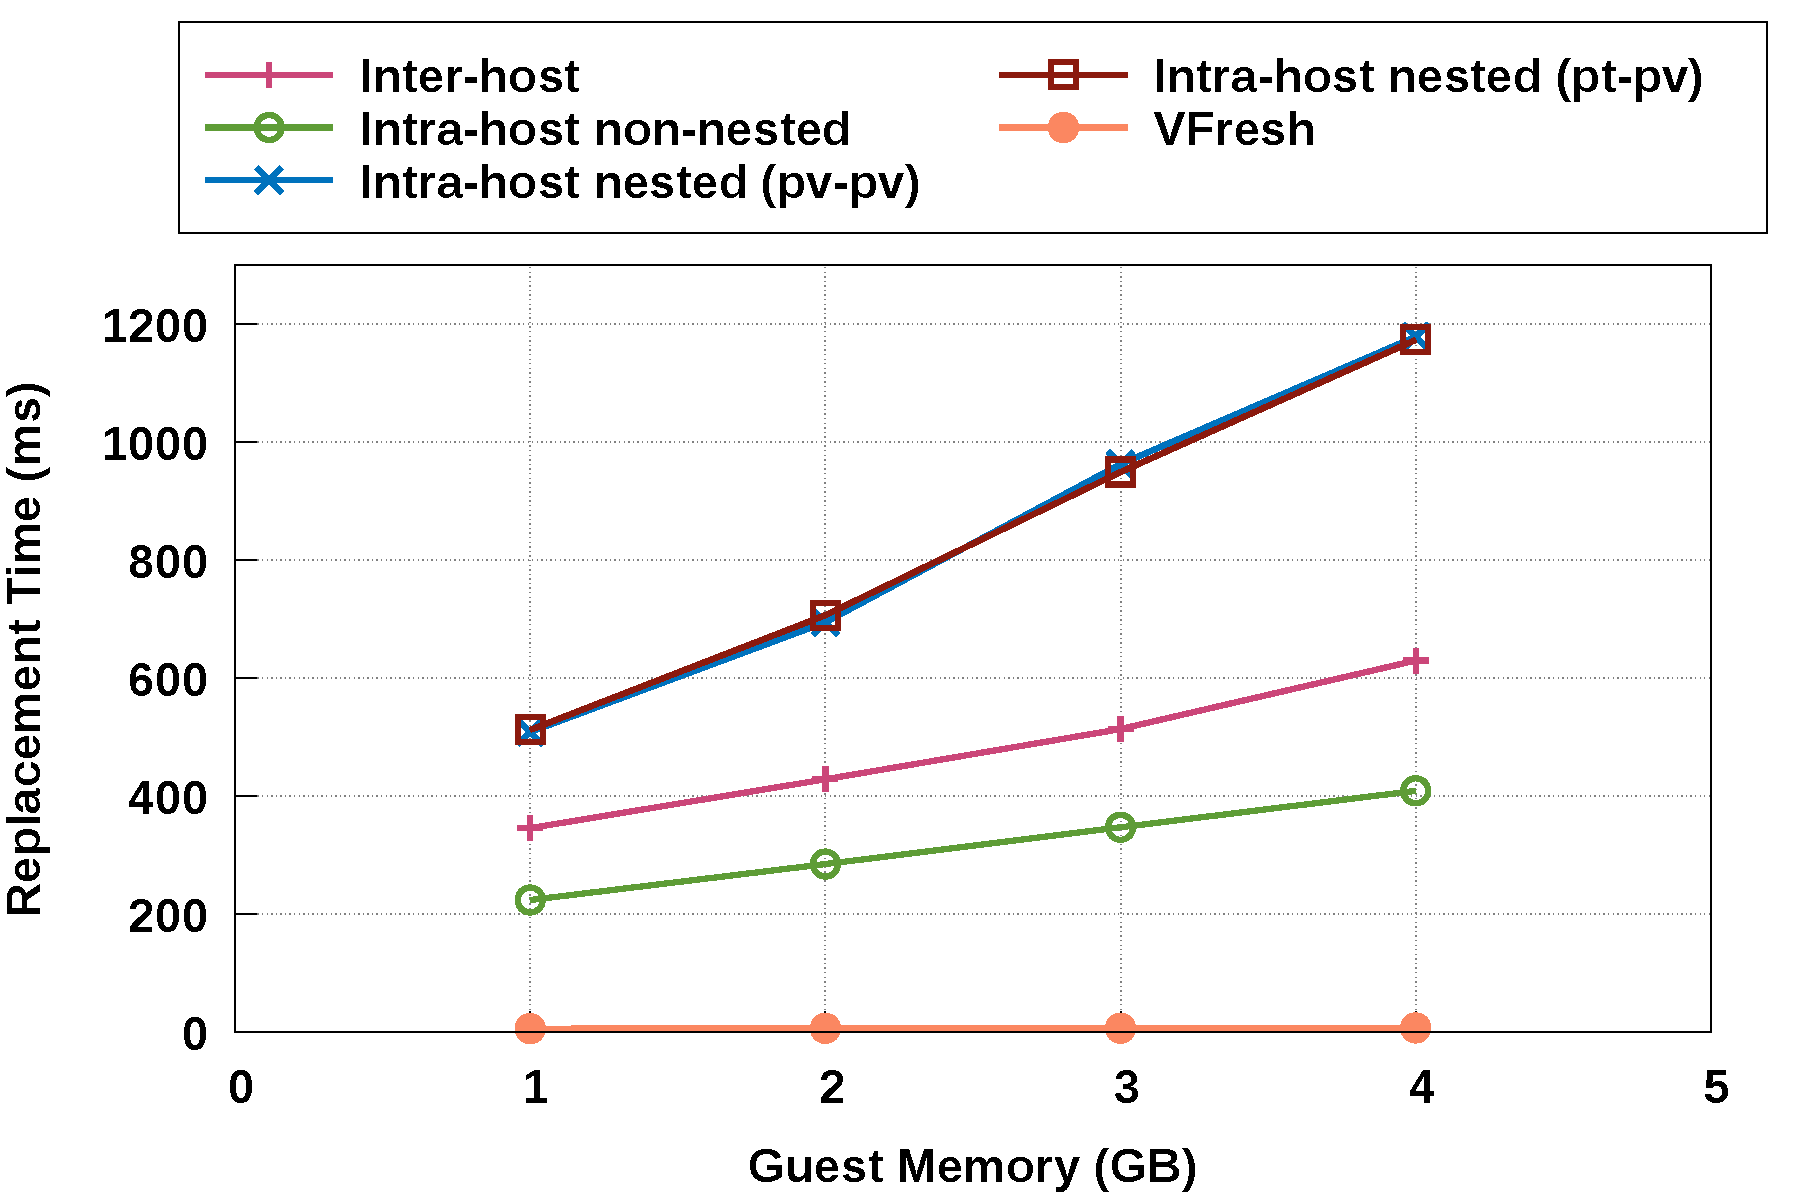
\includegraphics[width=0.45\textwidth]{figures/idle_guest_migration_with_vFresh.pdf}
%  \caption{Comparison of hypervisor replacement time for an idle guest with \arch and different setups.}
  %\caption{Comparison of refresh time for an idle guest - Our solution vs Optimized Pre-copy}
%  \label{fig:idleVfresh}
%  \includegraphics[width=15cm,height=6cm,keepaspectratio]{architecture__1_.jpg}
%\end{figure}

%\begin{figure}[t!]
%  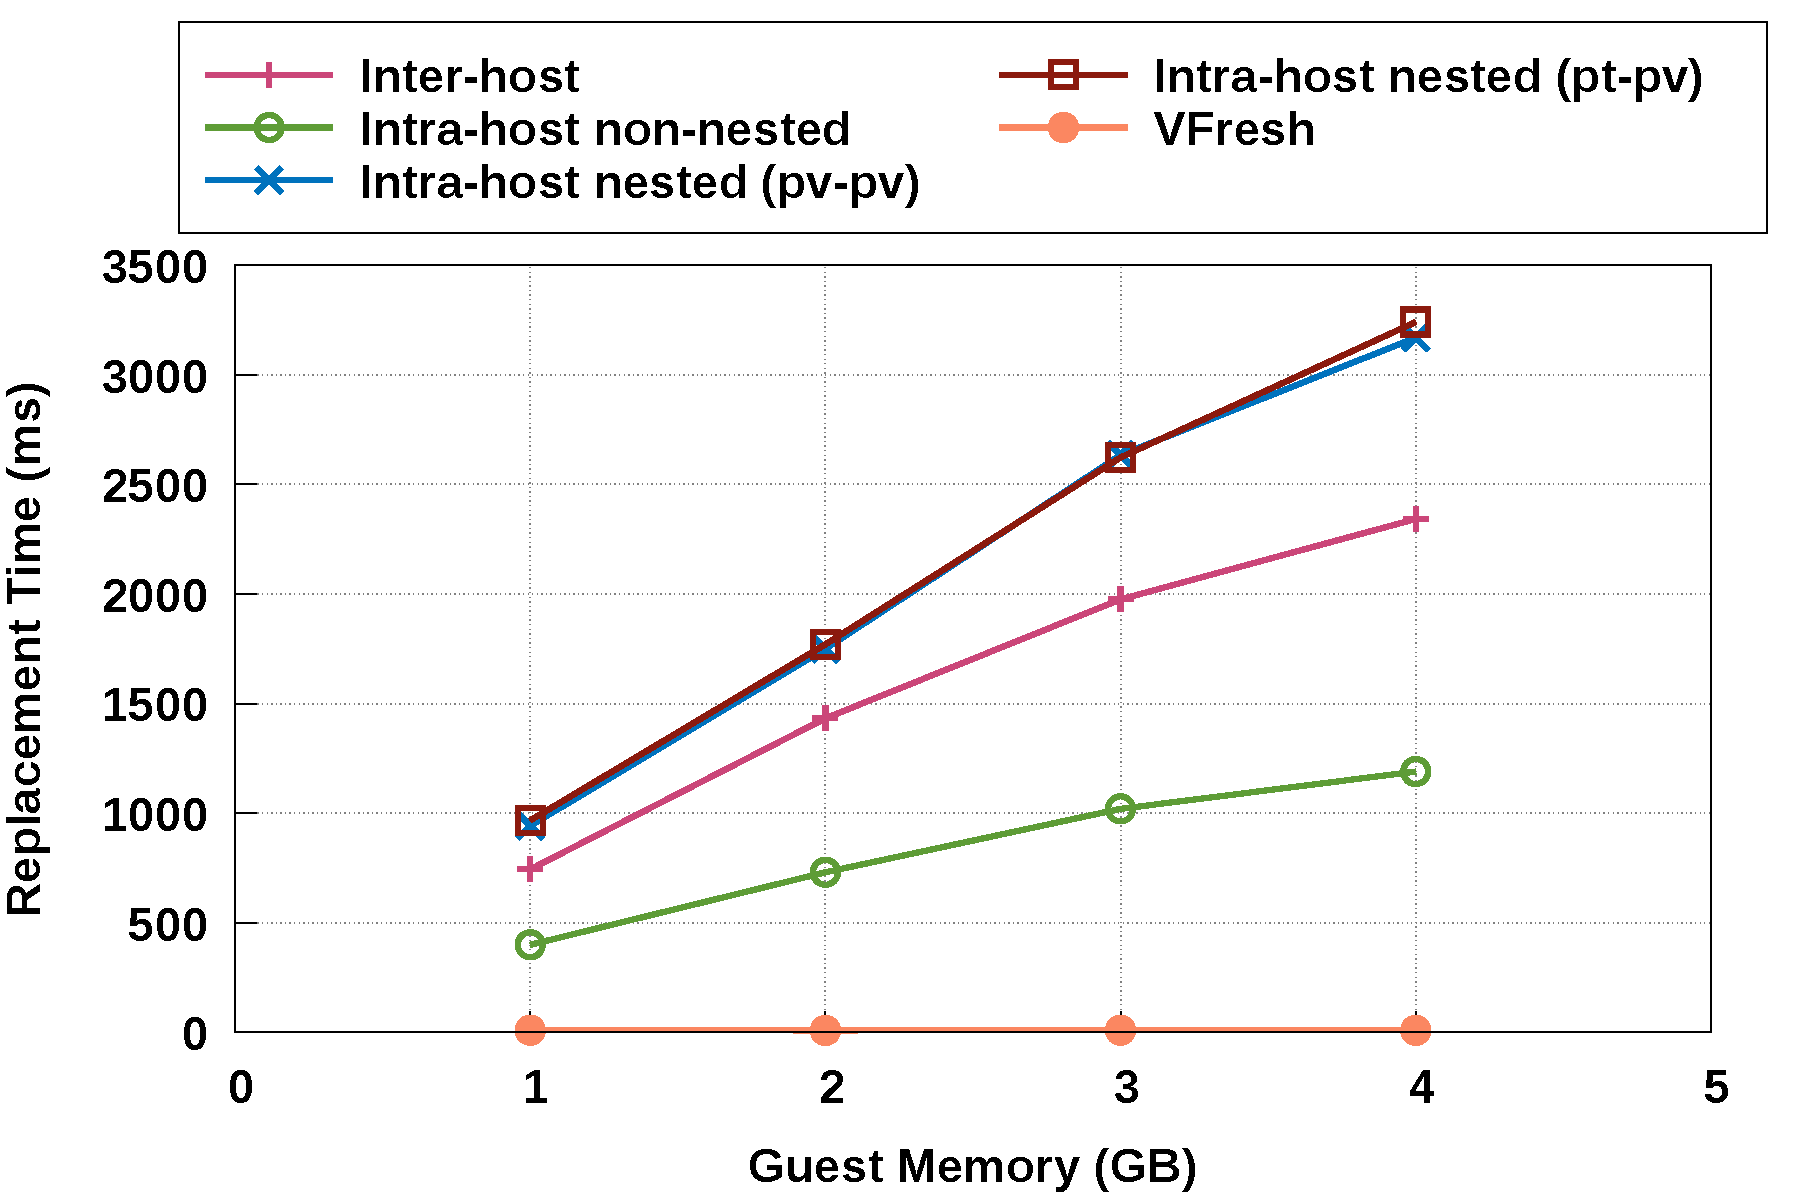
\includegraphics[width=0.45\textwidth]{figures/busy_guest_migration_with_vFresh.pdf}
%  \caption{Comparison of hypervisor replacement time for a guest performing write-intensive workloads with \arch and different setups.}
%  \label{fig:VfreshBusy}
%\end{figure}

%\begin{figure*}[t!]
% 	  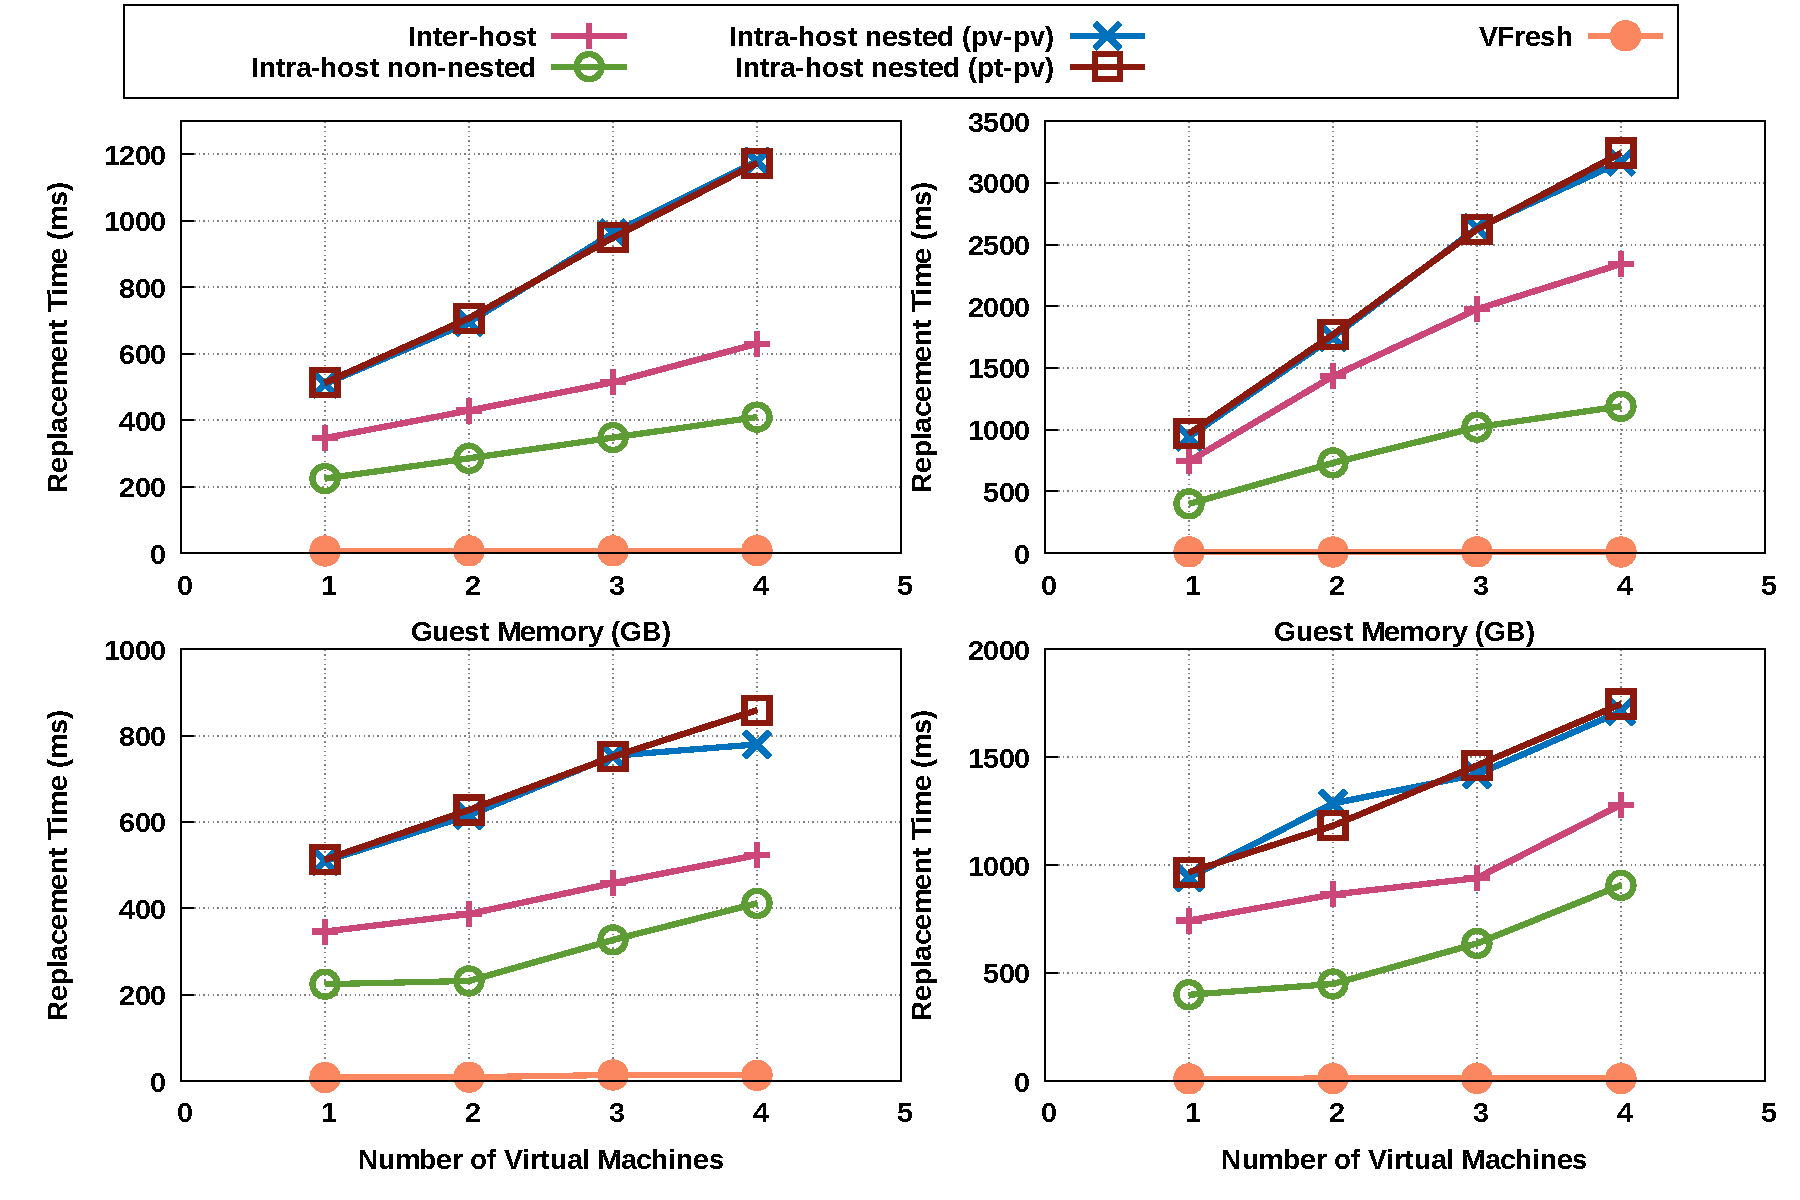
\includegraphics[width=0.98\textwidth]{figures/migration.pdf}
%  \caption{Architecture for hypervisor replacement with direct-device assignment and thin hyperplexor.}
%TODO: Please fix this caption
%  \label{fig:vFresharch}
  %\includegraphics[width=15cm,height=6cm,keepaspectratio]{architecture__1_.jpg}
%\end{figure*}

\begin{figure*}
\centering
\begin{minipage}{.43\textwidth}
  \centering
  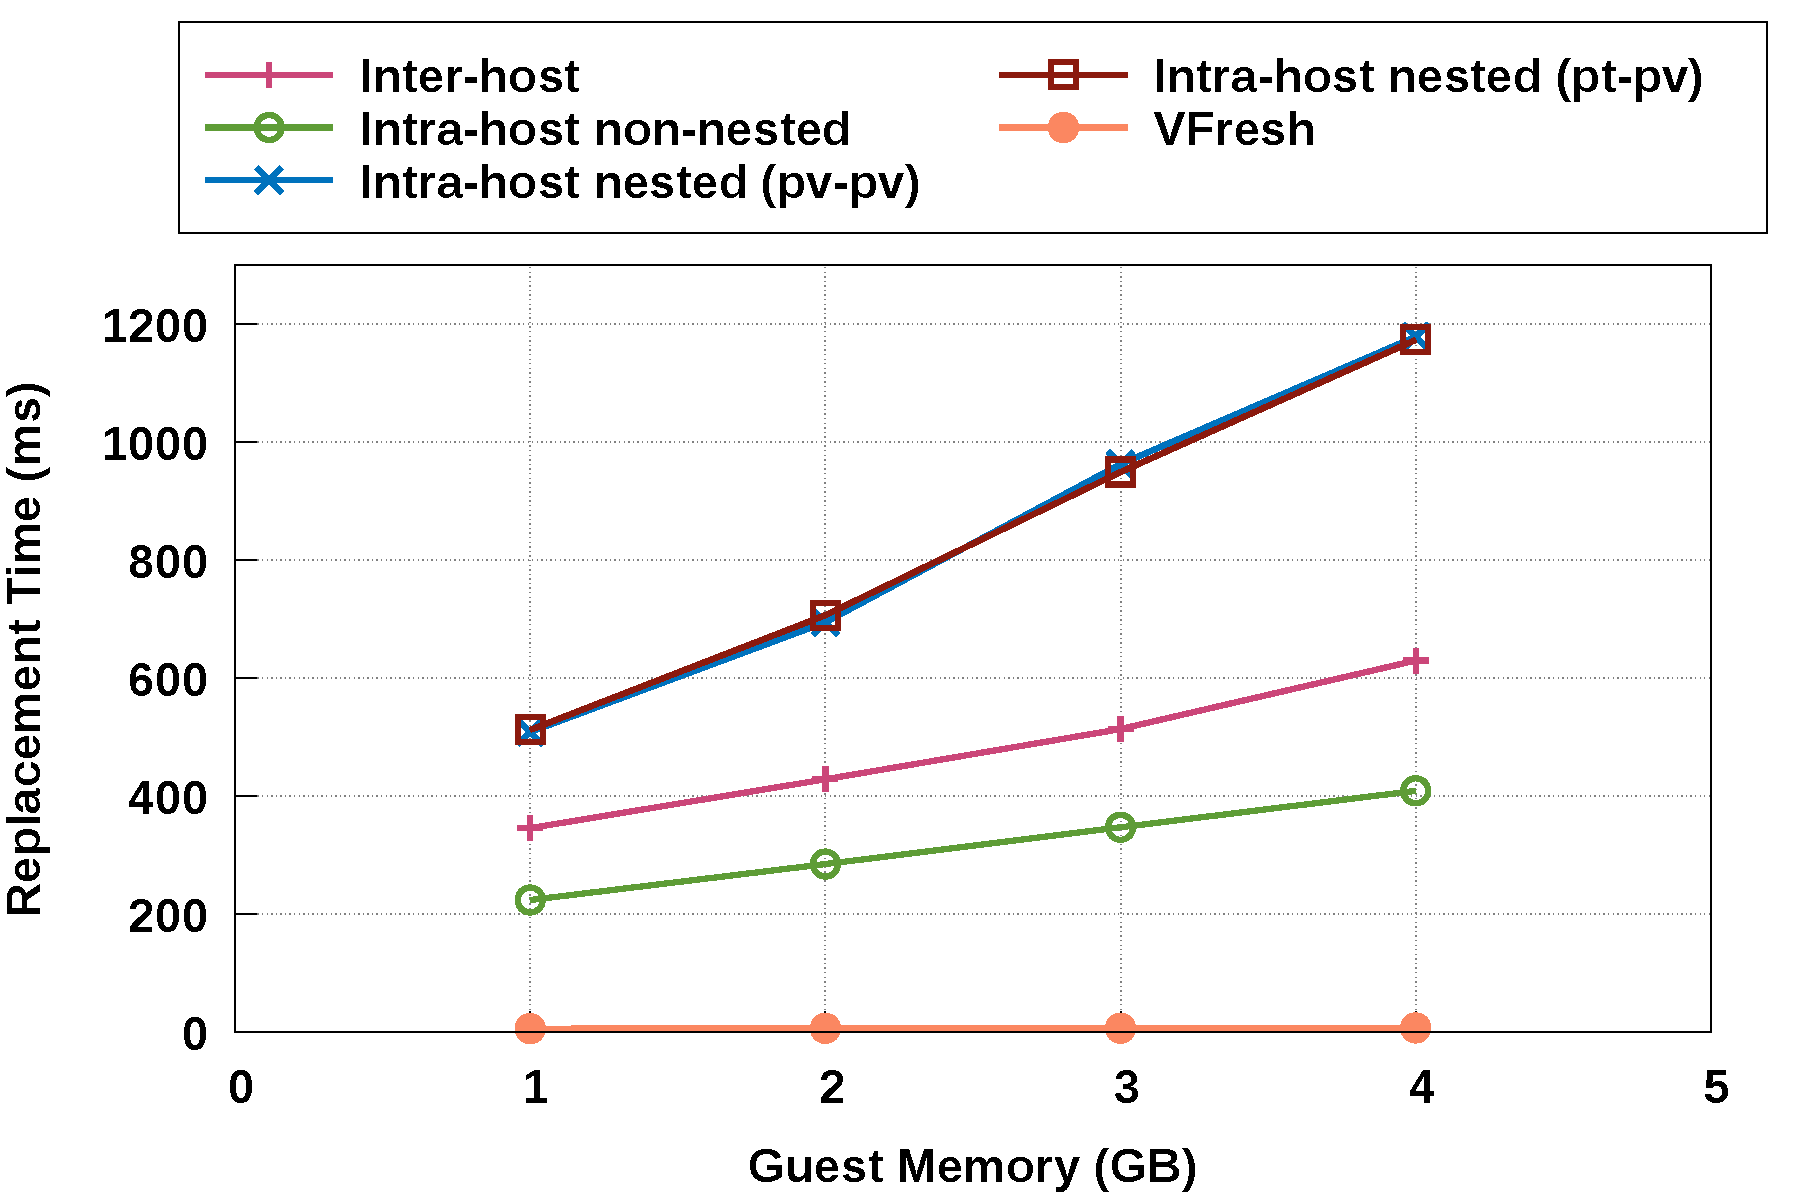
\includegraphics[width=.95\linewidth]{figures/idle_guest_migration_with_vFresh.pdf}
   \vspace{-0.1in}
  \captionof{figure}{Comparison of hypervisor replacement time for an idle VM with varying memory sizes.}
  \label{fig:idleVfresh}
\end{minipage}
\hspace{0.34in}
\begin{minipage}{.43\textwidth}
  \centering
  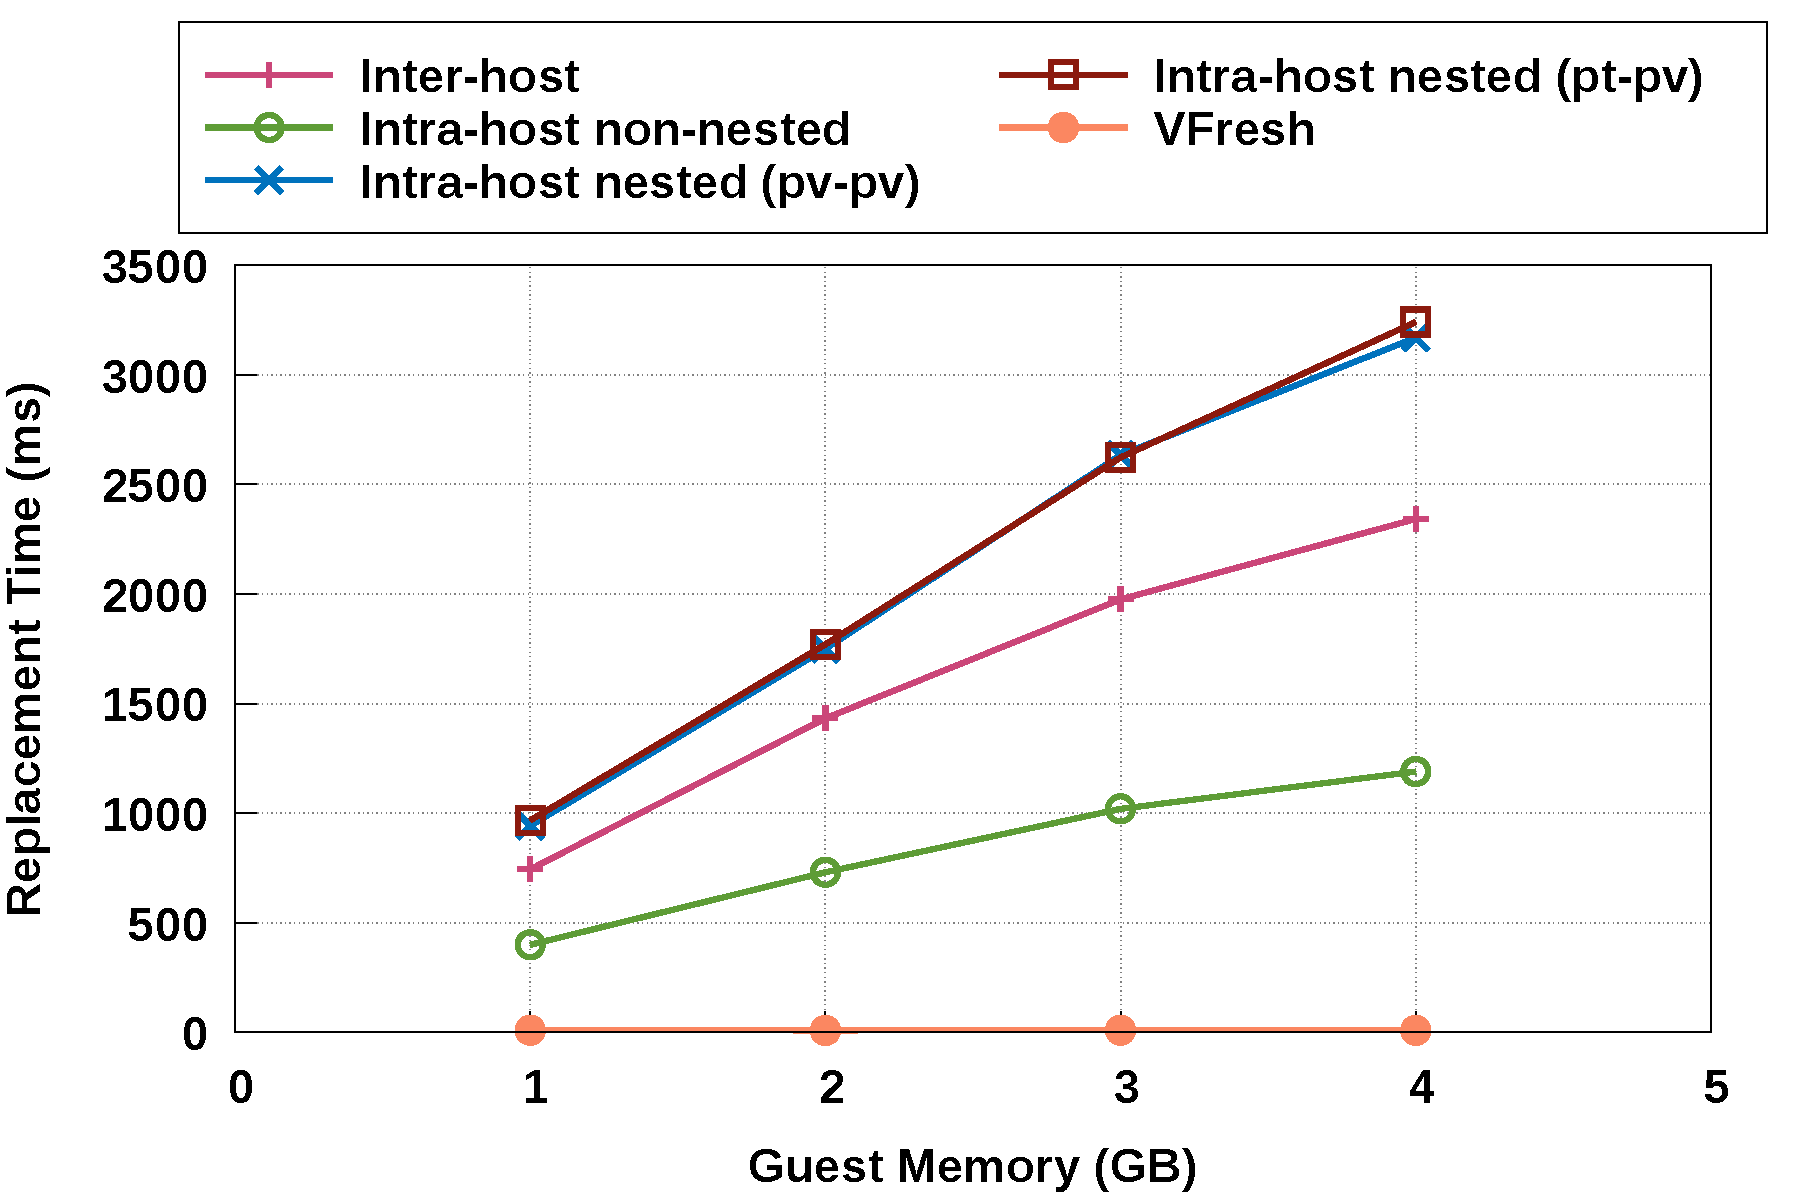
\includegraphics[width=.95\linewidth]{figures/busy_guest_migration_with_vFresh.pdf}
   \vspace{-0.1in}
  \captionof{figure}{Comparison of hypervisor replacement time for a write-intensive VM with varying memory sizes.}
  \label{fig:VfreshBusy}
\end{minipage}%
  \vspace{-0.1in}
\end{figure*}

\begin{figure*}
\centering
\begin{minipage}{.43\textwidth}
  \centering
  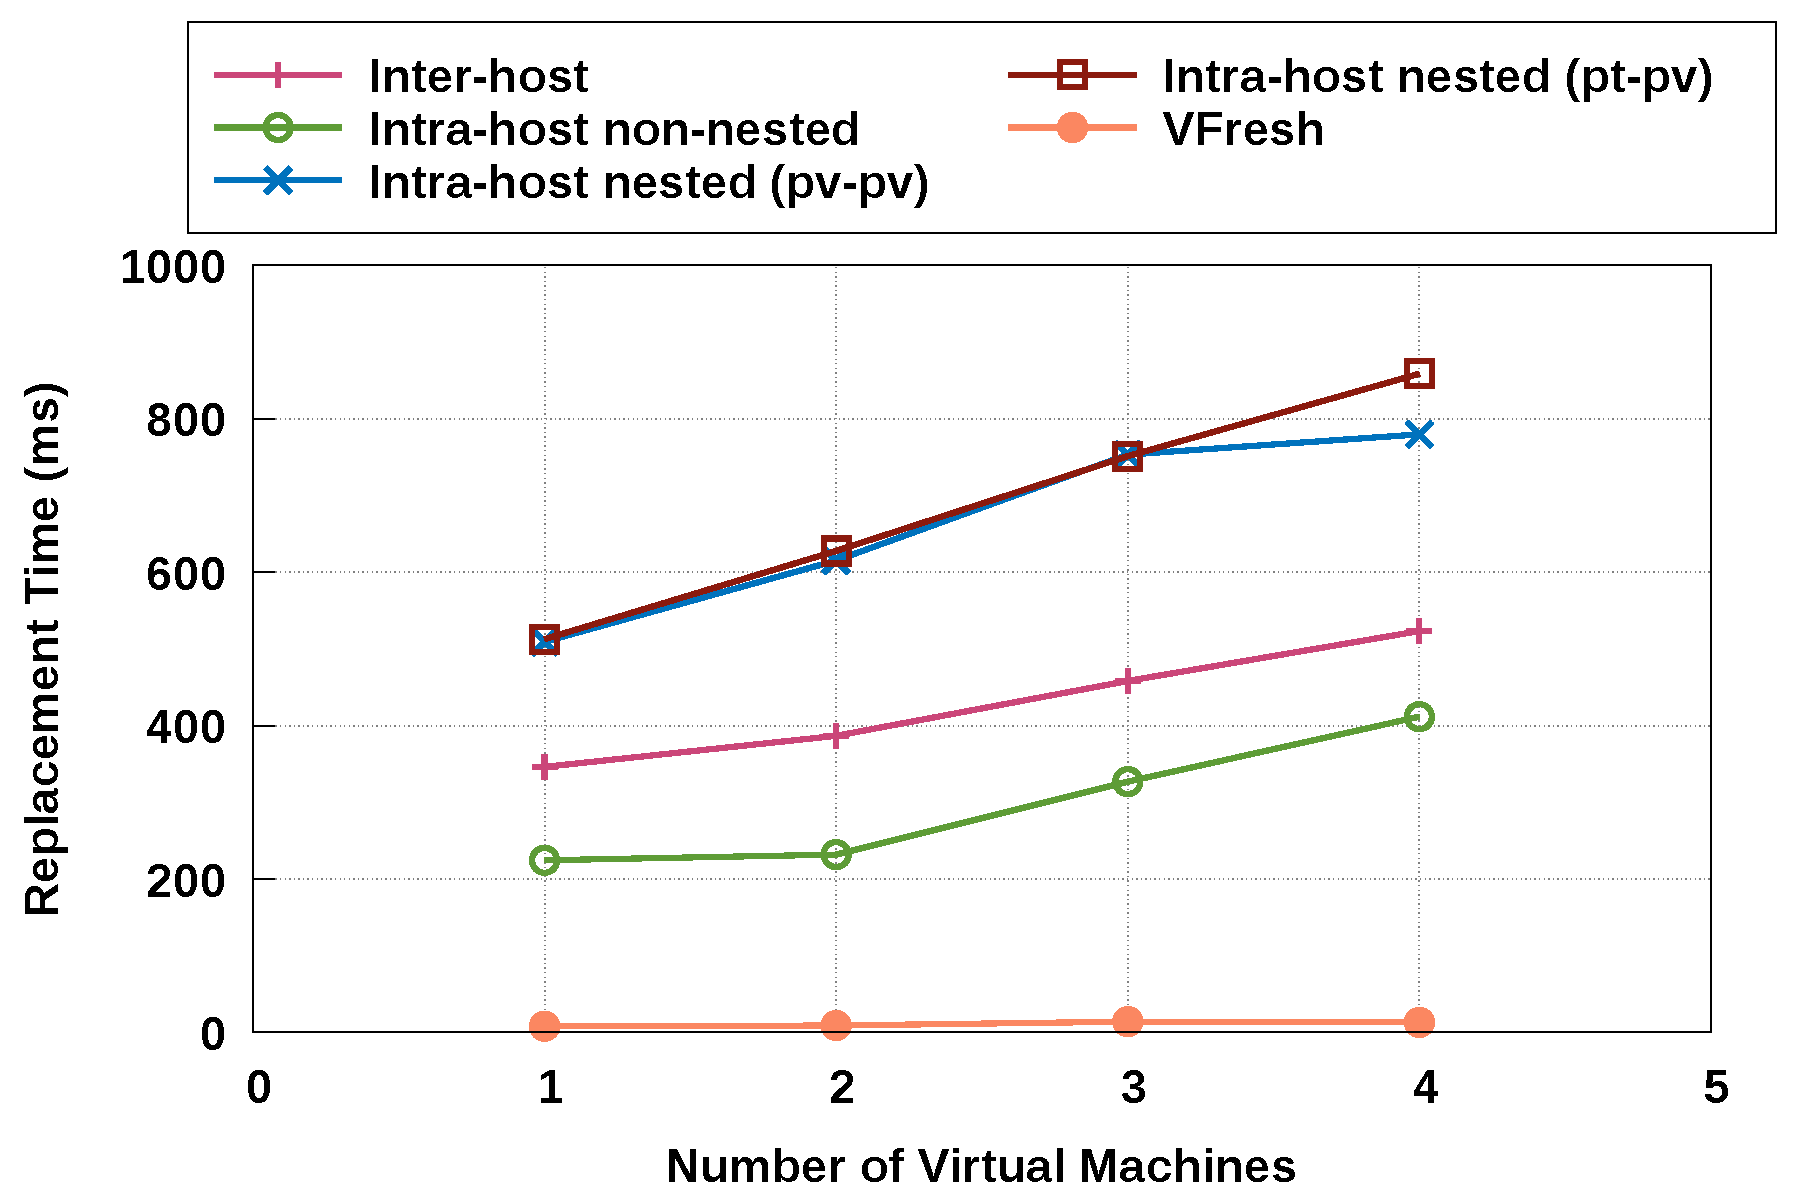
\includegraphics[width=.95\linewidth]{figures/multivm_idle_guest_migration_vFresh.pdf}
   \vspace{-0.1in}
  \captionof{figure}{Comparison of hypervisor replacement time for multiple idle VMs with varying VM \#.}
  \label{fig:multiVfreshIdle}
\end{minipage}
\hspace{0.34in}
\begin{minipage}{.43\textwidth}
  \centering
  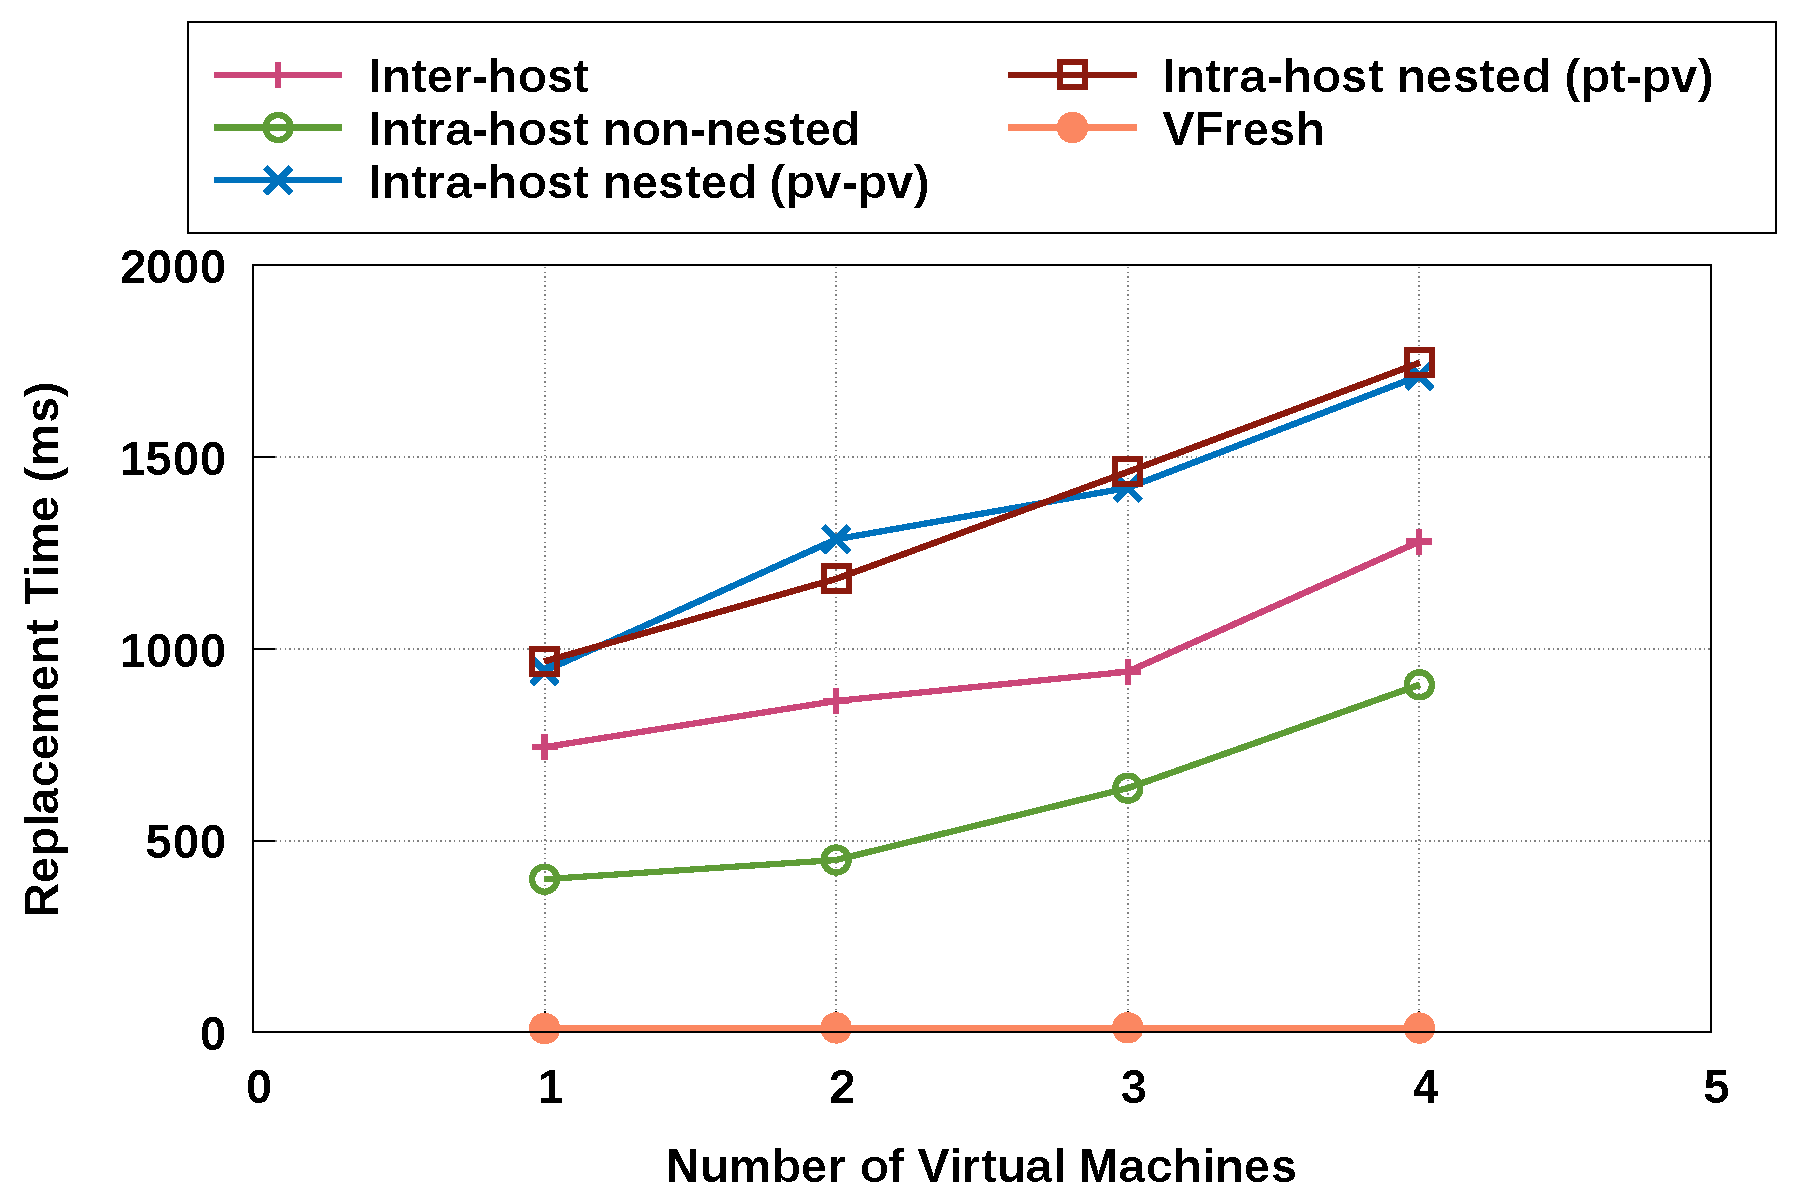
\includegraphics[width=.95\linewidth]{figures/multivm_busy_guest_migration_vFresh.pdf}
   \vspace{-0.1in}
  \captionof{figure}{Comparison of hypervisor replacement time for multiple write-intensive VMs with varying VM \#.}
  \label{fig:multiVfreshBusy}
\end{minipage}%
  \vspace{-0.1in}
\end{figure*}

\begin{table}
\small
\begin{tabular}{|p{1.75cm}|p{1.65cm}|p{1.5cm}|p{1.5cm}|} \hline
 & Hyperplexor & Hypervisor & Guest \\ \hline
Host & 1GB, \linebreak 1CPU & - & - \\ \hline
Non-Nested & 8GB, \linebreak 4CPUs & - & 1GB, 1VCPU \\ \hline
Nested & 32GB, 10CPUs & 8GB, \linebreak 4VCPUs & 1GB, 1VCPU \\ \hline
\arch & 32GB, 10CPUs & 8GB, \linebreak 4VCPUs & 1GB, 1VCPU \\ \hline
\end{tabular}
\vspace{6pt}
\caption{Experiment setup to measure the hypervisor replacement time for different setups.}
\label{tab:setup1}
\end{table}


\subsubsection{Replacement Time}
We measure the hypervisor replacement time under \arch and compare it with 
%optimized pre-copy migration. 
the four cases based on the optimized pre-copy live migration as stated in Section \ref{sec:motiv}, which are (a) inter-host, (b) intra-host nested (pv-pv), (c) intra-host nested (pt-pv), and (d) intra-host non-nested. The nested virtualization configurations are listed in detail in Table \ref{tab:setup1}: The L2 VMs are configured with 1 VCPU (and varying memory sizes under different test cases); the L1 hypervisors are configured with 8 GB memory and 4 VCPUs; and the L0 hyperplexor is configured with 32 GB memory and 10 CPUs. 

\para{Single VM.} First, we use a single idle VM and vary its memory sizes from 1 GB to 4 GB. \fref{fig:idleVfresh} shows that the total replacement time under the inter-host case is around 0.35 seconds for 1 GB memory and 0.6 seconds for 4 GB memory. Under the intra-host nested cases (both pv-pv and pt-pv), the replacement time increases to around 0.5 seconds for 1 GB memory, and 1.17 seconds for 4 GB memory. In contrast, the total hypervisor replacement time under \arch is extremely low --- 10 ms. Further, the replacement time remains constant as the VM's memory size increases. It is because, in \arch, the memory is re-mapped between the L1 hypervisors and such operations are performed out of the critical path of the VM state transfer; the replacement time only comprises of the time of transferring the VCPU and I/O device state information, which is constant. 
%the total replacement time is almost constant and independent of the VM memory size. Instead, the replacement time only comprises of the time of transferring the VCPU and I/O device state information. 
%The migration rate limit, pre-copy iterations and the page dirty rate do not affect the total migration time in \arch.  
However, under both the inter-host and intra-host cases, transferring the memory pages through the network accounts for higher total migration time and thus higher replacement time. 

%Explain what is working set
%dirty page rate is 50000pages/second
Next, we use a busy VM with varying memory sizes. The busy VM runs a ``working set'' benchmark which dirties the memory at a controllable page dirty rate --- we fix it as 5,000 pages per second in all our experiments.
%As explained before, working set is a write-intensive synthetic benchmark 
%with varying sizes of memory at a fixed dirty rate --- 5,000 pages per second. \
In \fref{fig:VfreshBusy}, under all pre-copy live migration based cases the replacement time again increases as the memory size of the VM increases. The replacement time is higher than that under the idle VM, because dirtied pages are transferred in multiple rounds for the busy VM.
With \arch, the replacement time remains constant irrespective of the memory dirty rate --- the replacement time remains around 10 ms for the cases with varying memory sizes.
%with increase in size of the working set as the number of dirty pages to be transferred in pre-copy iterations increase. 
%The increase in total migration time for nested guest is due to the overhead introduced by nested virtualization. 

%Busy guest	Memory Variation			
%							1		2		3		4
%Inter-host					743.6	1433	1975.8	2342.6
%Intrahost non-nested		399.6	730.6	1020	1190
%Intrahost nested(pv-pv)	942.4	1750	2634	3170
%Intrahost nested(pv-pt)	967.4	1770.6	2623.2	3241.6
%Hyperfresh					10		9		10.2	9.4


%\begin{figure}
%	\centering
%	\subfloat[Idle guest]{
%		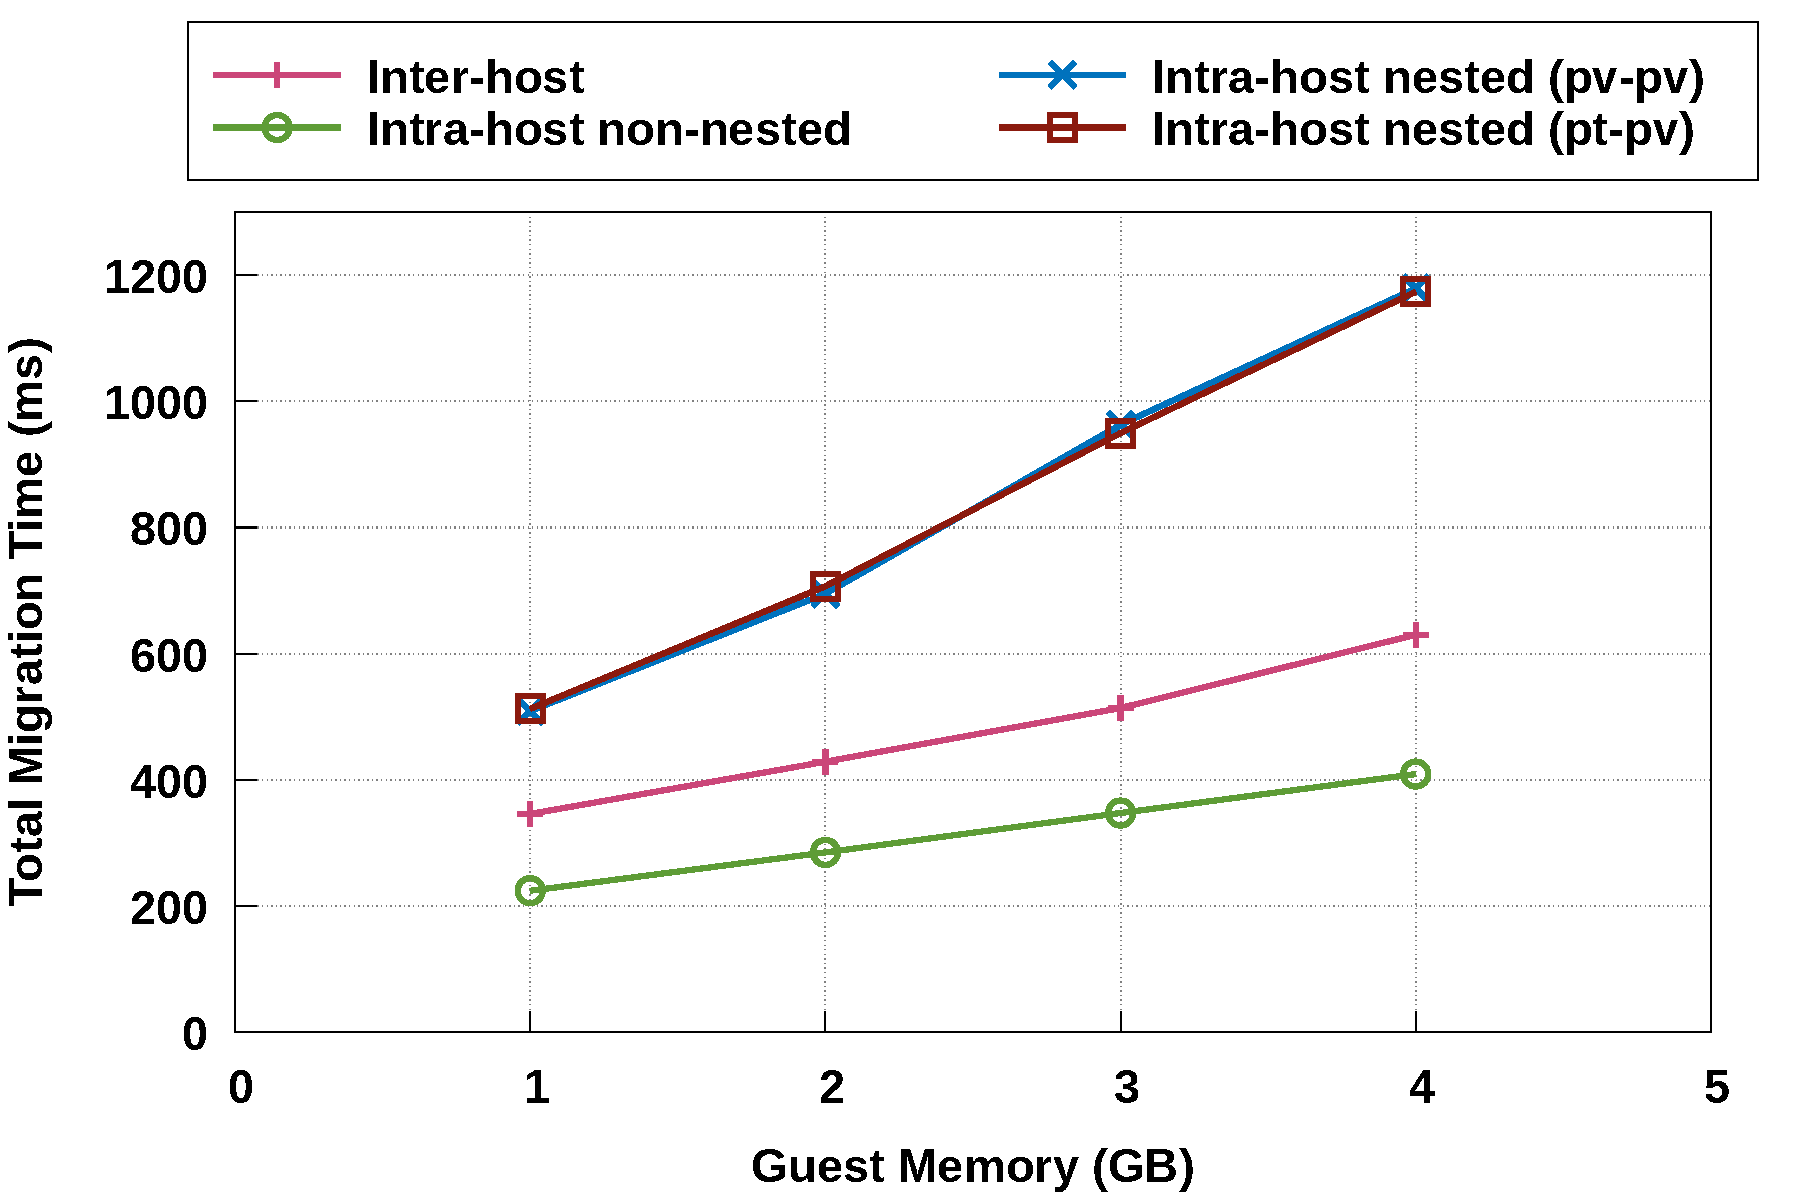
\includegraphics[width=.235\textwidth]{figures/idle_guest_migration.pdf}}
%	\subfloat[Busy guest]{
%		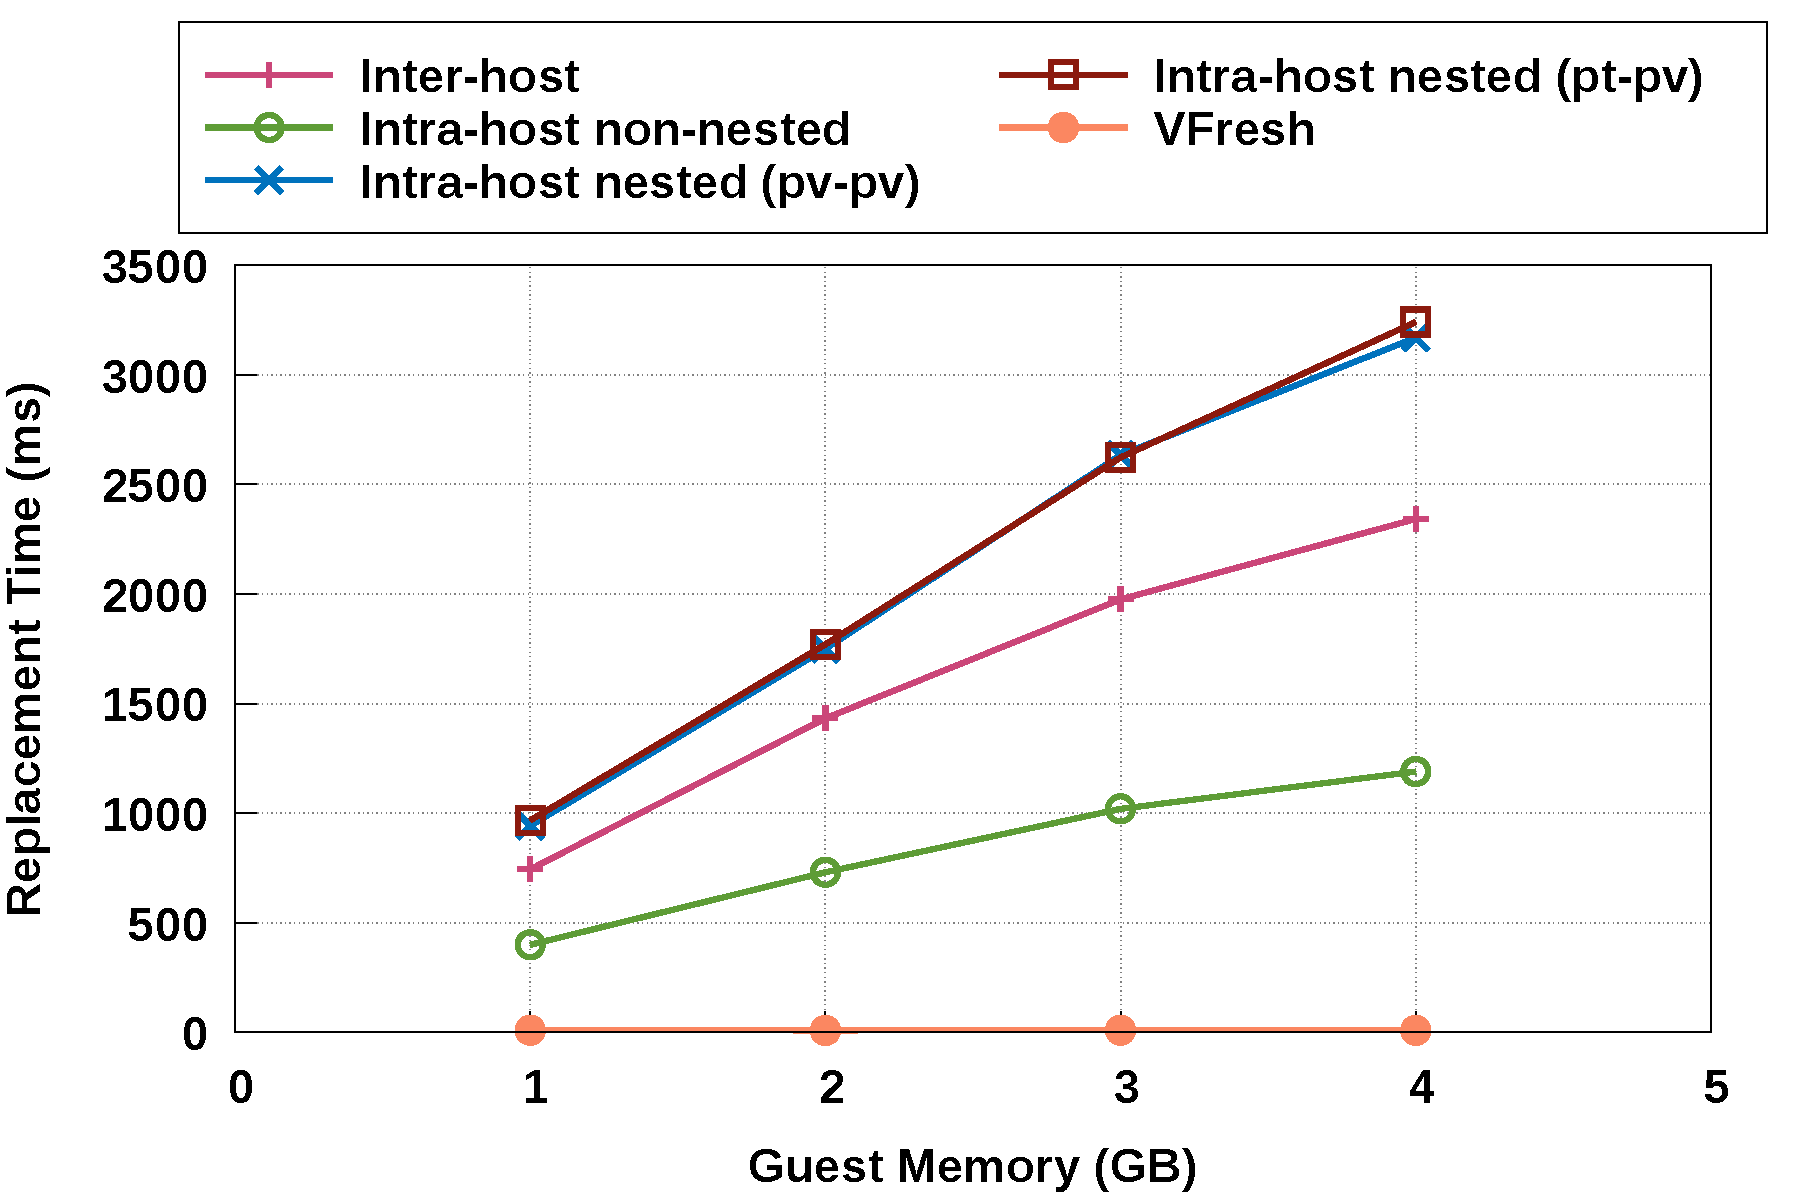
\includegraphics[width=.235\textwidth]{figures/busy_guest_migration_with_vFresh.pdf}}
%	\caption{Replacement time comparison with VFresh}
%	\label{fig:rt_exp1}
%\end{figure}

\para{Multiple VMs.} 
Further, we measure the replacement time
%to replace old hypervisor with new hypervisor that is 
by running multiple VMs on the same stale hypervisor and later moving them to another co-located replacement hypervisor. We vary the VM number from 1 to 4. 
Each VM is configured with 1 GB memory; all the VMs start the migration at the same time. 
We consider the following two cases: (1) with all VMs being idle and (2) with all VMs being busy (with the same page dirty rate of 5,000 pages per second). 

In \fref{fig:multiVfreshIdle}, with all idle VMs, it takes 0.3 seconds to migrate 1 VM and 0.5 seconds to migrate 4 VMs under inter-host live migration. The migration time increases to 0.5 seconds for migrating 1 VM and 0.8 seconds for 4 VMs under intra-host nested live migration (for both pv-pv and pt-pv setups). In \fref{fig:multiVfreshBusy}, with all busy VMs, it takes 0.7 seconds to migrate 1 VM and 1.27 seconds for 4 VMs under inter-host live migration. Under intra-host nested live migration (for both pv-pv and pt-pv setups), the migration time increases to 1 second for 1 VM and 1.75 seconds for 4 VMs.
In contrast, with \arch, the time to replace the hypervisor remains 10 ms with either idle or busy VMs. The replacement time does not increase as the number of VMs increases, because again the VMs' memory is remapped and only the VCPU and I/O device state is transferred during hypervisor replacement.
%from one host to another using optimized pre-copy and it takes 0.3s to migrate 1 VM and increases to 0.5s to migrate 4 virtual machines. The migration time increases when nested virtual machines are migrated from one hypervisor to another on the same host with both pv-pv and pt-pv setup. 
%In \fref{fig:multiVfreshBusy}, 
%we migrate virtual machines that perform write intensive workload. Every virtual machine dirties the memory at the rate 50000 pages/second. The virtual machines are migrated once 80\% of every VM's memory is dirtied simultaneously. The migration time for optimized pre-copy migration increases from 0.7 s to 1.27 s for 1 VM to 4 VMs. In \arch, the time to replace the hypervisor remains to be 10ms running busy or idle virtual machines. The replacement time does not increase with increase in number of virtual machines because the guest memory is co-mapped and only the VCPU and I/O device information is transferred during migration.

\begin{figure}
	\centering
	\subfloat[Optimized pre-copy]{
		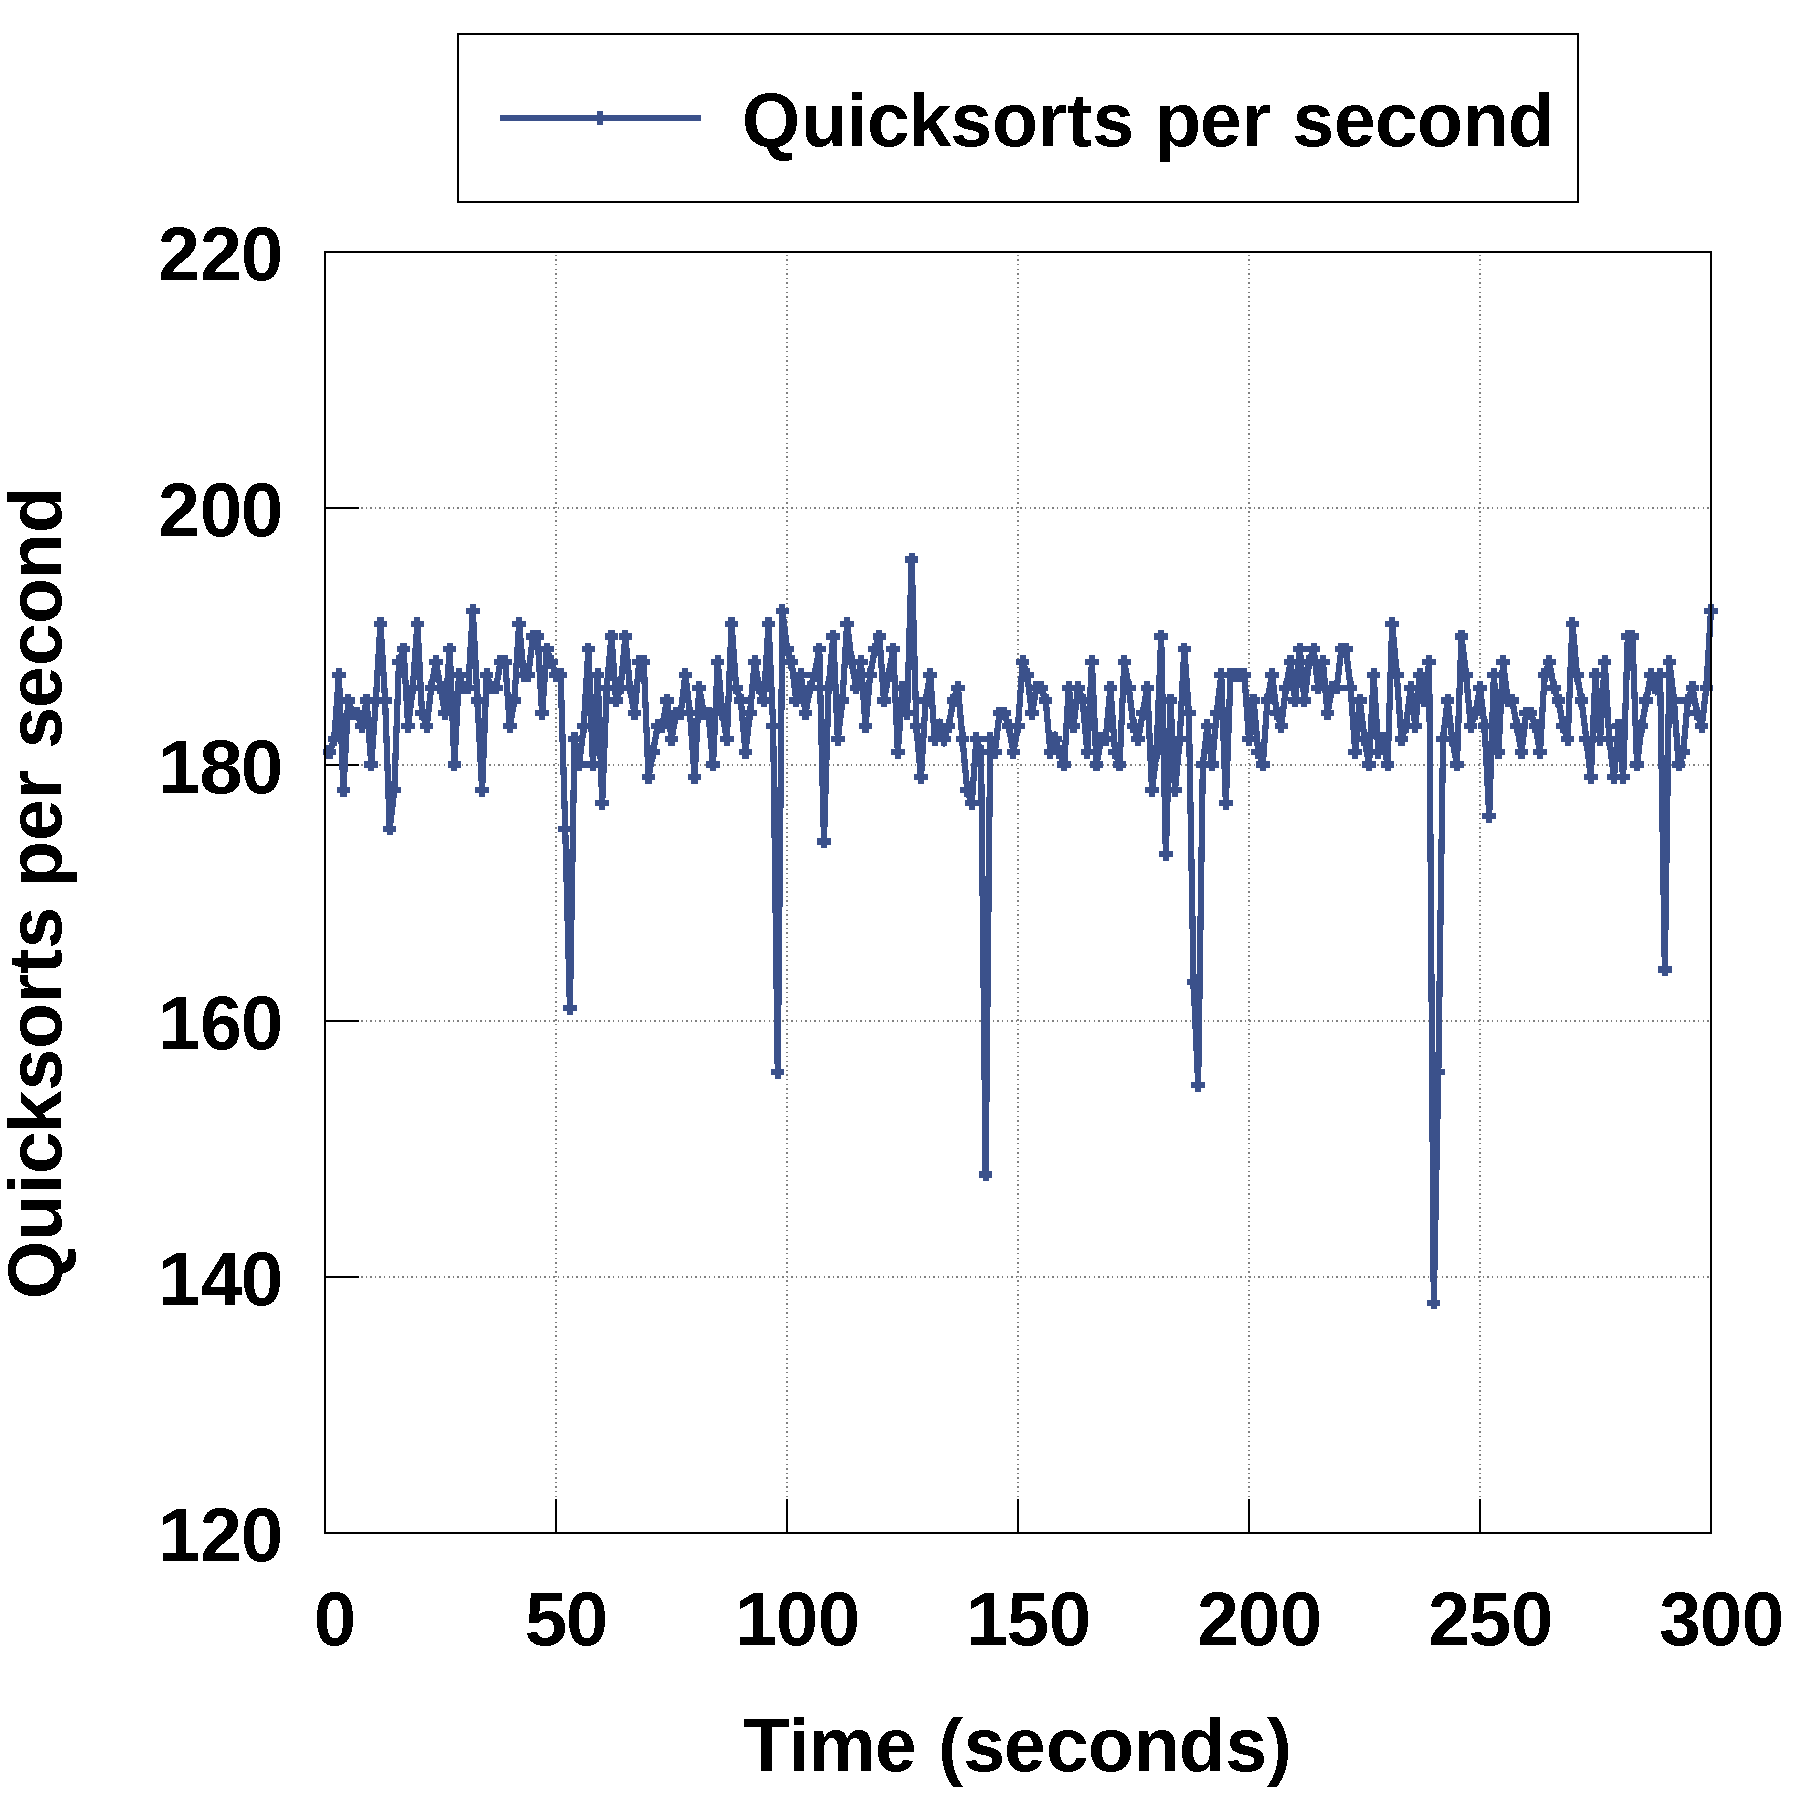
\includegraphics[width=.235\textwidth]{figures/qsortps_1GB_nested_precopy_disable_rate_limit.pdf}}
	\subfloat[\arch.]{
		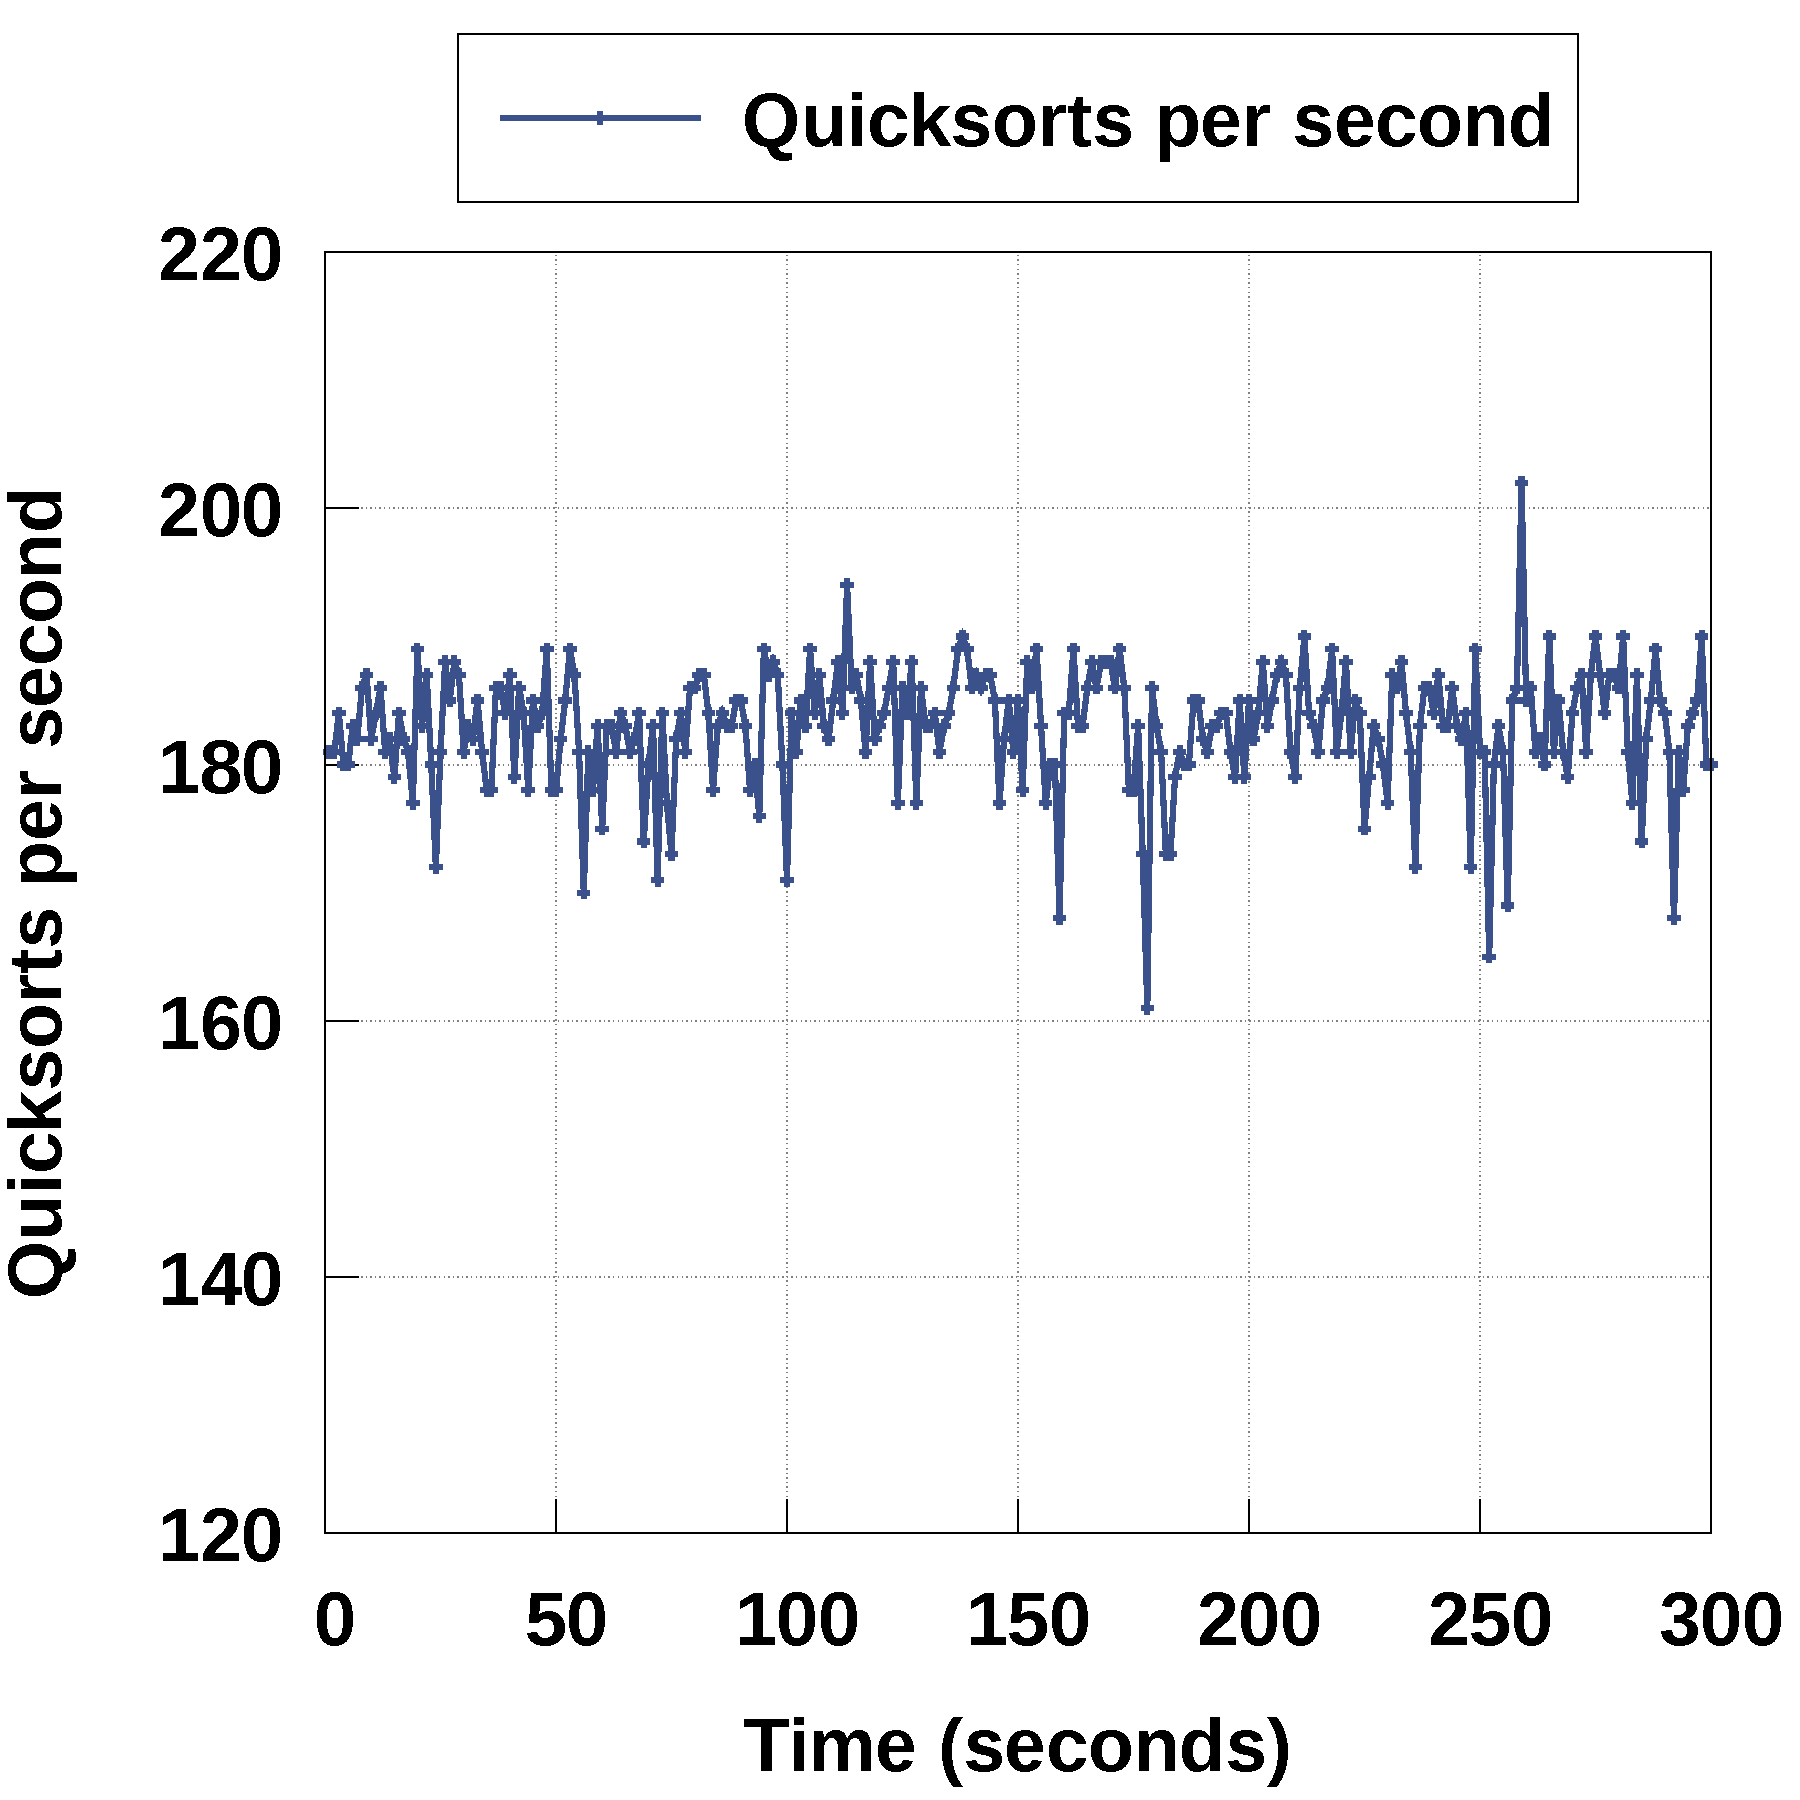
\includegraphics[width=.235\textwidth]{figures/qsortps_1GB_nested_precopy_hyperfresh.pdf}}
	\caption{Quicksort performance over multiple hypervisor replacements.}
	\label{fig:implq}
\end{figure}


%\begin{figure}
%	\centering
%   	\subfloat[Optimized Pre-copy migration]{
%		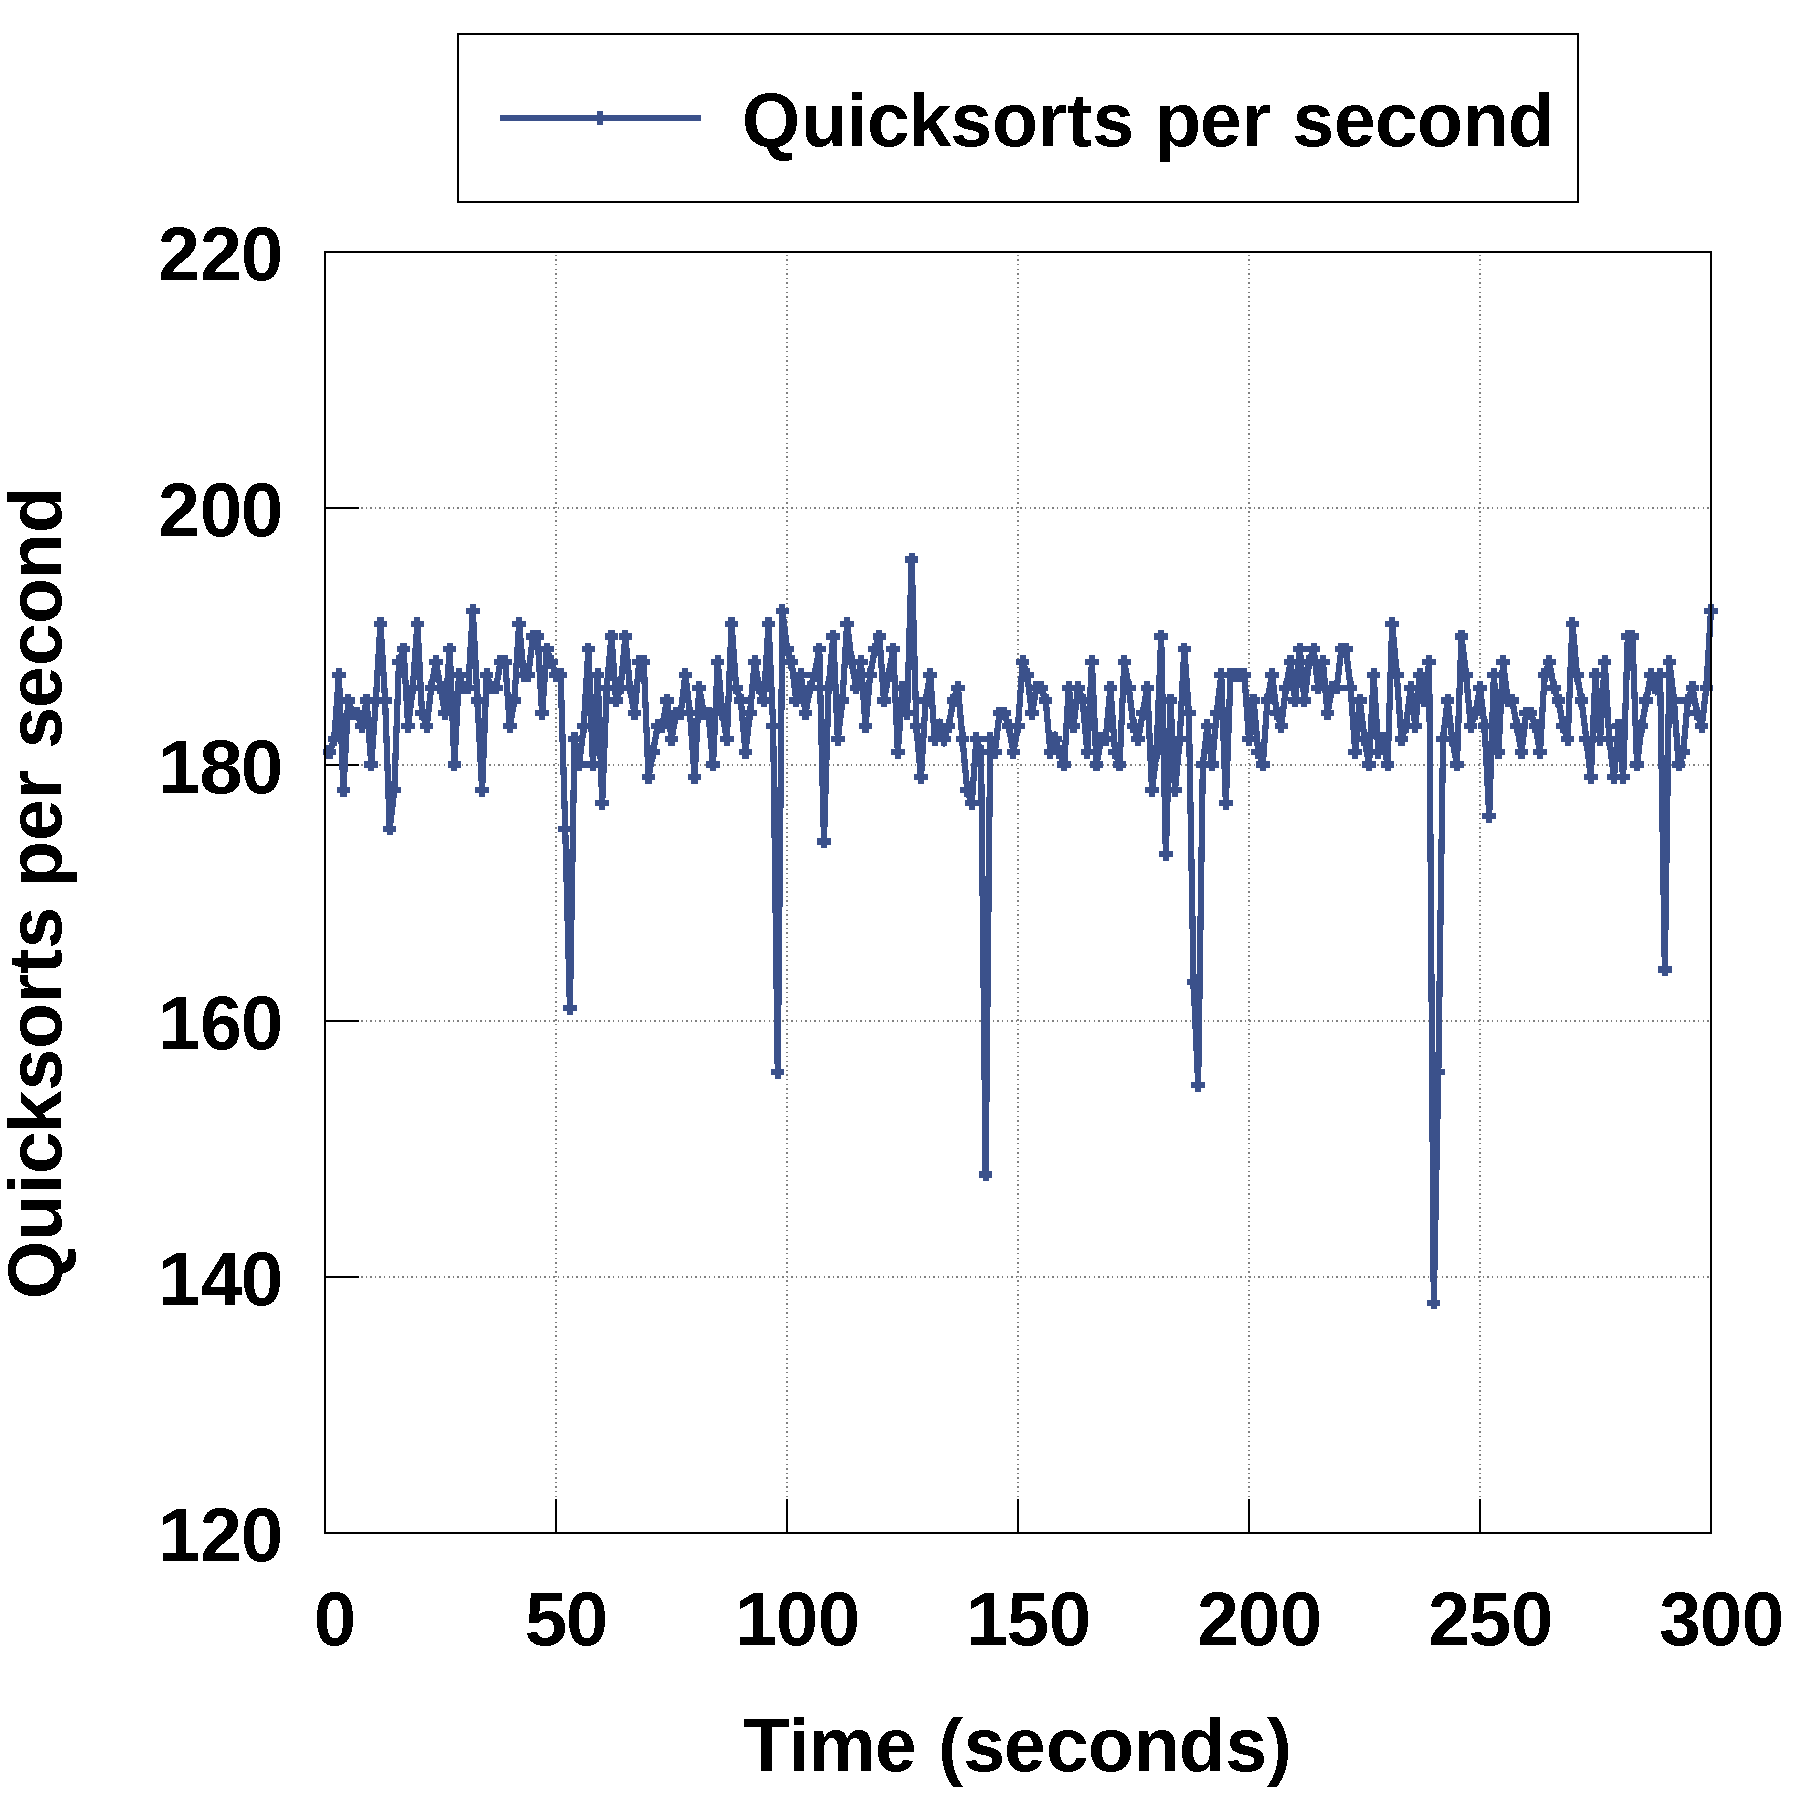
\includegraphics[width=.235\textwidth]{figures/qsortps_1GB_nested_precopy_disable_rate_limit.pdf}}
%		\hspace{0.1in}     
%	\subfloat[\arch]{
%		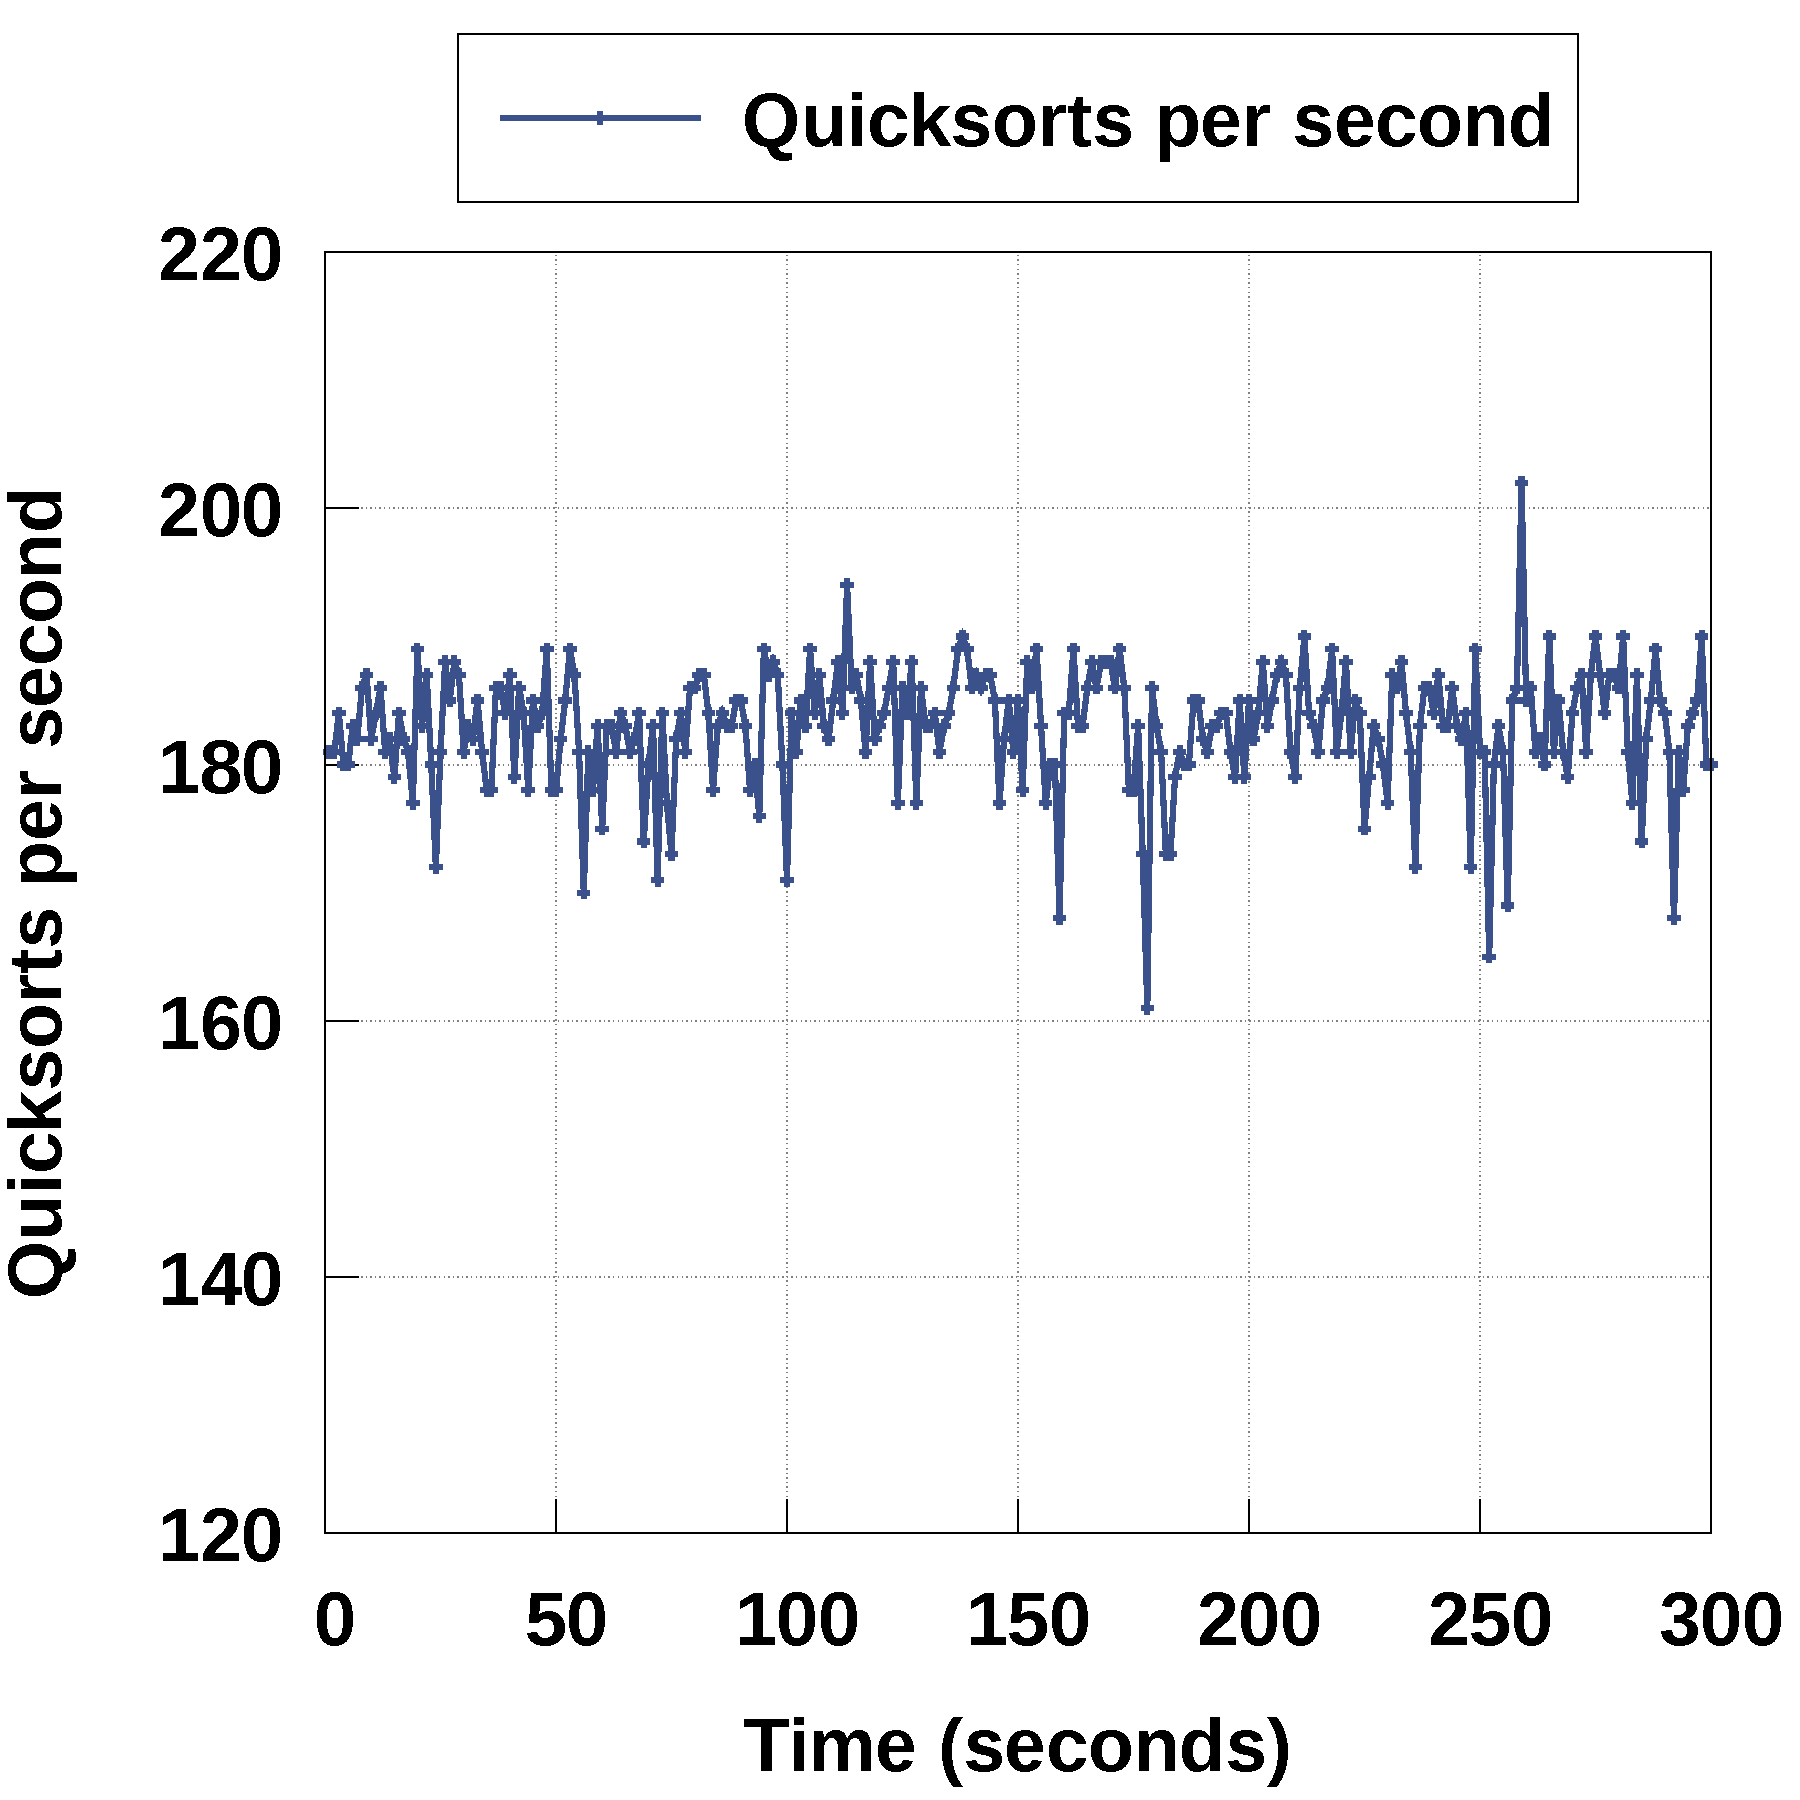
\includegraphics[width=.235\textwidth]{figures/qsortps_1GB_nested_precopy_hyperfresh.pdf}}
		%\hspace{0.1in}
%		\vspace{-0.1in}
%	\caption{Quicksort performance during migration of a nested guest: Optimized Pre-copy vs. VFresh}
%	\vspace{-0.1in}
%    \label{fig:impl}
%\end{figure}

\subsubsection{Performance Impact} 
We measure the application performance during hypervisor replacement between \arch and the intra-host nested (pt-pv) case. We use a CPU-intensive benchmark, Quicksort.
%The Quicksort benchmark is a CPU-intensive benchmark: 
Quicksort first allocates 1 GB memory, and then each operation takes 200 KB (50 pages) from the pre-allocated memory, writes random integers into it and performs the quicksort algorithm on these pages. In \fref{fig:implq}, we conduct 6 hypervisor replacements over a 300-second time window for both \arch and the intra-host nested case. We measure the number of quicksort operations per second during both regular execution and replacement.
%during migration of a nested VM using \arch and compare the results nested optimized pre-copy live migration.

%Idle guest	Number of Vms variation			
%Guest Memory (GB)			1		2		3		4
%Inter-host					346.2	386.6	458.2	523.2
%Intrahost non-nested		224.4	231.8	326.8	411.6
%Intrahost nested (pv-pv)	509.2	615.2	753.2	779.6
%Intrahost nested (pv-pt)	512.6	627.6	751.2	858.6
%Hyperfresh					8		9		14		13

%\begin{figure}[t!]
%  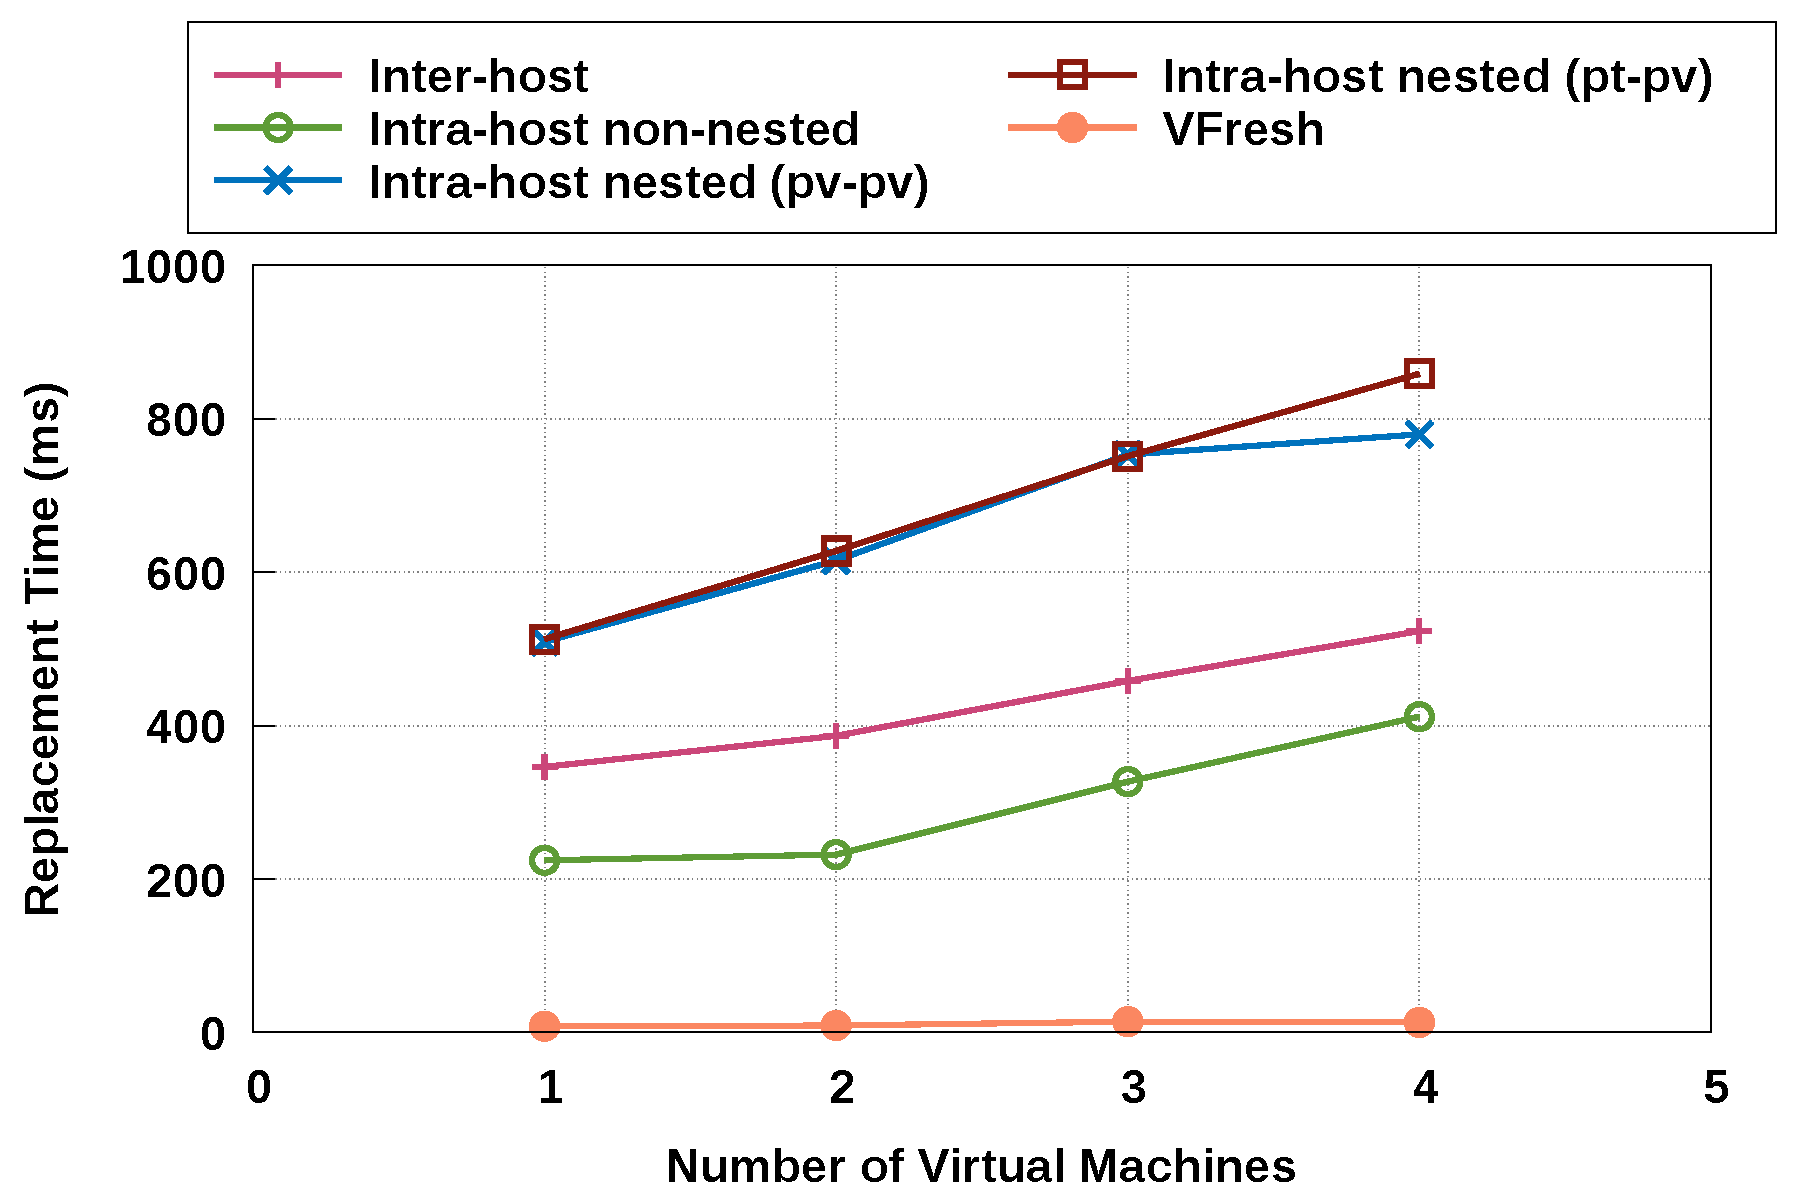
\includegraphics[width=0.45\textwidth]{figures/multivm_idle_guest_migration_vFresh.pdf}
%  \caption{Comparison of hypervisor replacement time for mutiple idle VMs with \arch and different setups.}
%  \label{fig:multiVfreshIdle}
%\end{figure}

%passthrough-vhost-net
%\fref{fig:impl1} shows that the performance of quicksort during optimized pre-copy migration. With optimized pre-copy, as the rate limit is disabled, a large number of dirty memory pages are transferred in less number of pre-copy iterations. As the number of pre-copy iterations decrease 
As shown in \fref{fig:implq}a, in the intra-host nested (pt-pv) case, there is no significant performance degradation during pre-copy iterations. However, the sharp performance dip is observed during the stop-and-copy phase, during which the VM is paused. 
%\fref{fig:impl}a. shows the dip in performance of quicksort during multiple optimized pre-copy migrations. 
In \fref{fig:implq}b, with \arch, the performance of quicksort does not reduce during the whole replacement and no significant performance dip is observed during the stop-and-copy phase. It is because, unlike the intra-host live migration case, \arch does not transfer any pages in the stop-and-copy phase, leading to much shorter stop-and-copy phase and hence less performance impact.   
%due to memory remapping


%Explain performance of quicksort during migration

%As discussed in the motivation section, the performance of the applications running in the guest decreases with decrease in the migration link bandwidth and the increase in bandwidth introduces significant network traffic during migration. In our solution, we eliminated the page transfer over the network and hence maintaining the performance of the applications in the guest. In Fig. 11 the performance of benchmark X does not get affected significantly during hypervisor refresh. 

%\begin{figure}[t!]
%  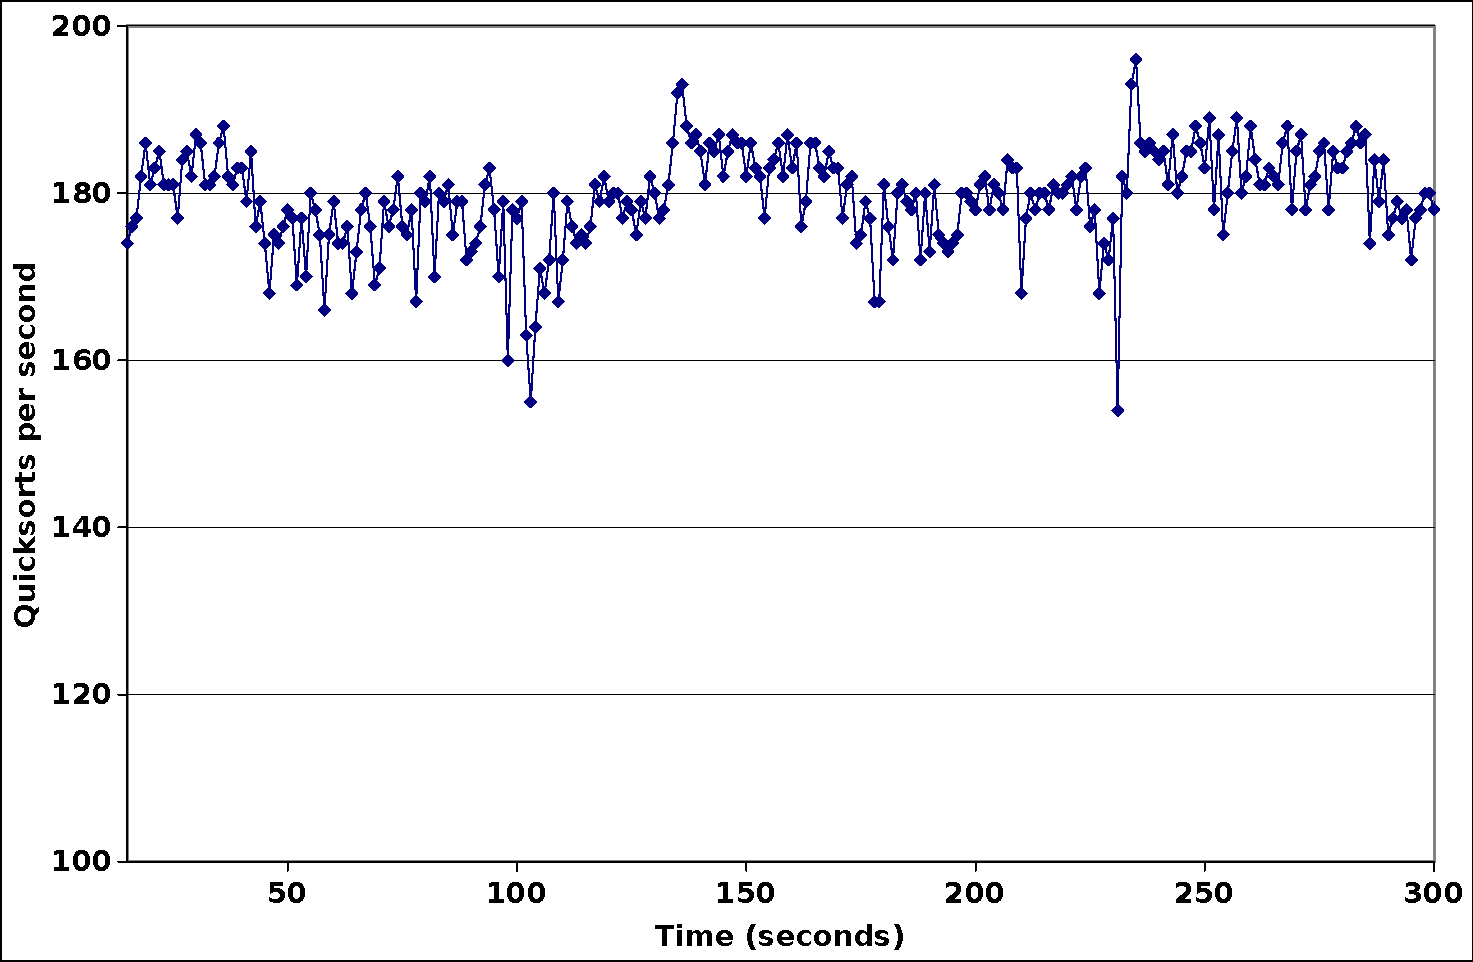
\includegraphics[width=0.5\textwidth]{figures/precopy-nested-2G-qsortps.pdf}
%  \caption{Pre-copy live migration: Performance of quicksort during migration of a %nested guest}
%  \label{quicksort-performance-1GB-nested-vhost-vhost.png}
%\end{figure}

%\subsubsection{Memory Mappings}
%The guest pages are pinned to the memory and populate the EPT and shadow EPT entries on boot up. The time taken to pin the pages in memory and populate the page table entries on the source host are 1.7 s, 3.3  s, 4.8 s, 6.3 s for a 1 GB, 2 GB, 3 GB and 4 GB memory respectively. The time taken on the destination host is 0.56 s, 1.2 s, 1.6 s, 2 s for 1 GB, 2 GB, 3 GB and 4GB respectively. The memory mapping time increases with increase in memory size of the guest as the number of pages to be mapped and hence the page table entries to be populated increase. The memory-mapping time measured represent the time taken to create the grant table used to transfer the memory mappings. The time taken to create the grant table increase with increase in guest memory as the number of hypercalls from hypervisor to hyperplexor increase along with grant table entries. However, this does not affect the total migration time as the grant table is created during the VM boot process.


%\begin{figure}[t!]
%  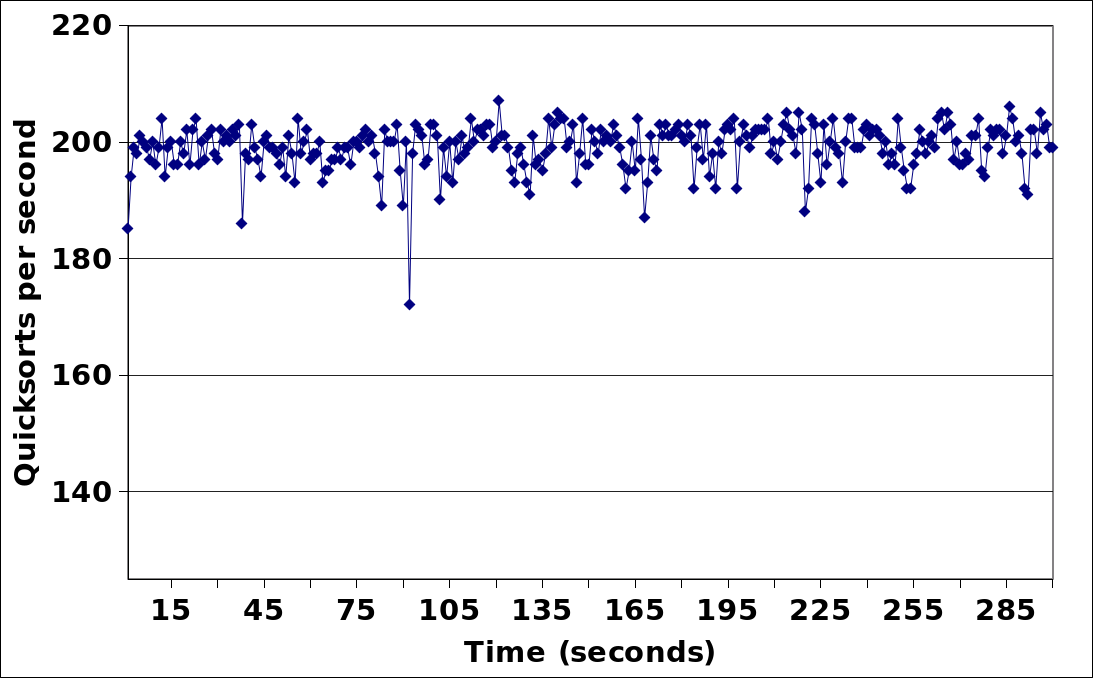
\includegraphics[width=0.5\textwidth]{figures/inter-host-quicksort-1GB.png}
%  \caption{Performance of quicksort during migration of guest from one host to another}
%  \label{quicksort-performance-1GB-interhost}
%  %\includegraphics[width=15cm,height=6cm,keepaspectratio]{architecture__1_.jpg}
%\end{figure}

%\begin{figure}[t!]
%  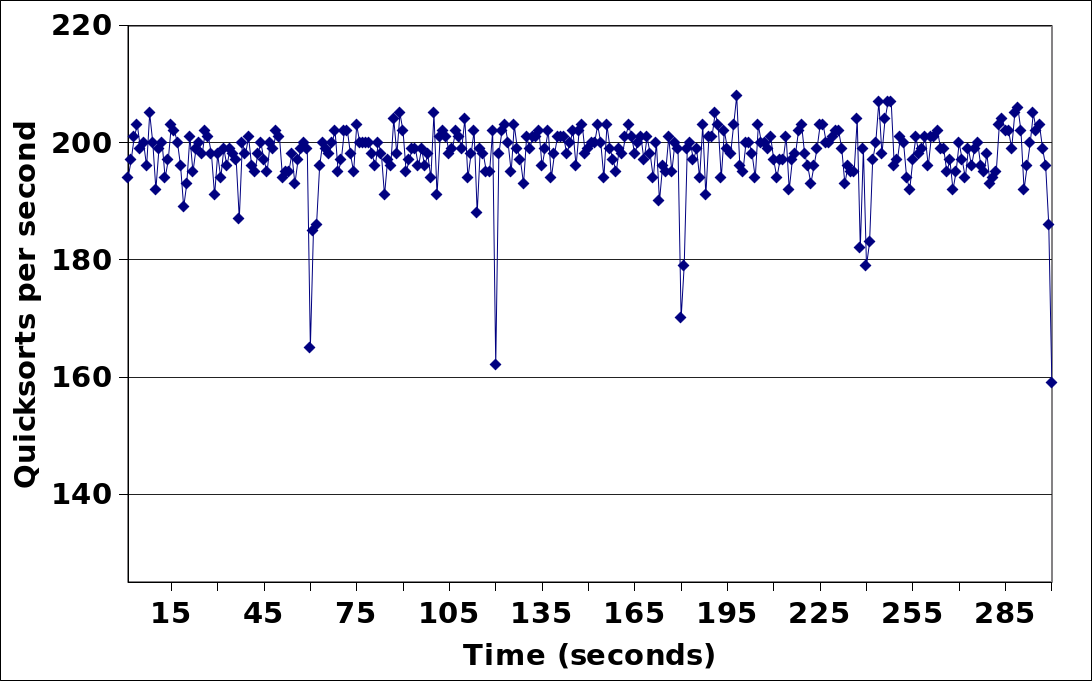
\includegraphics[width=0.5\textwidth]{figures/intrahost-non-nested-quicksort-1GB.png}
%  \caption{Performance of quicksort during migration of non-nested guest on same host}
%  \label{quicksort-performance-1GB-intrahost.png}
%  %\includegraphics[width=15cm,height=6cm,keepaspectratio]{architecture__1_.jpg}
%\end{figure}

%\begin{figure}[t!]
%  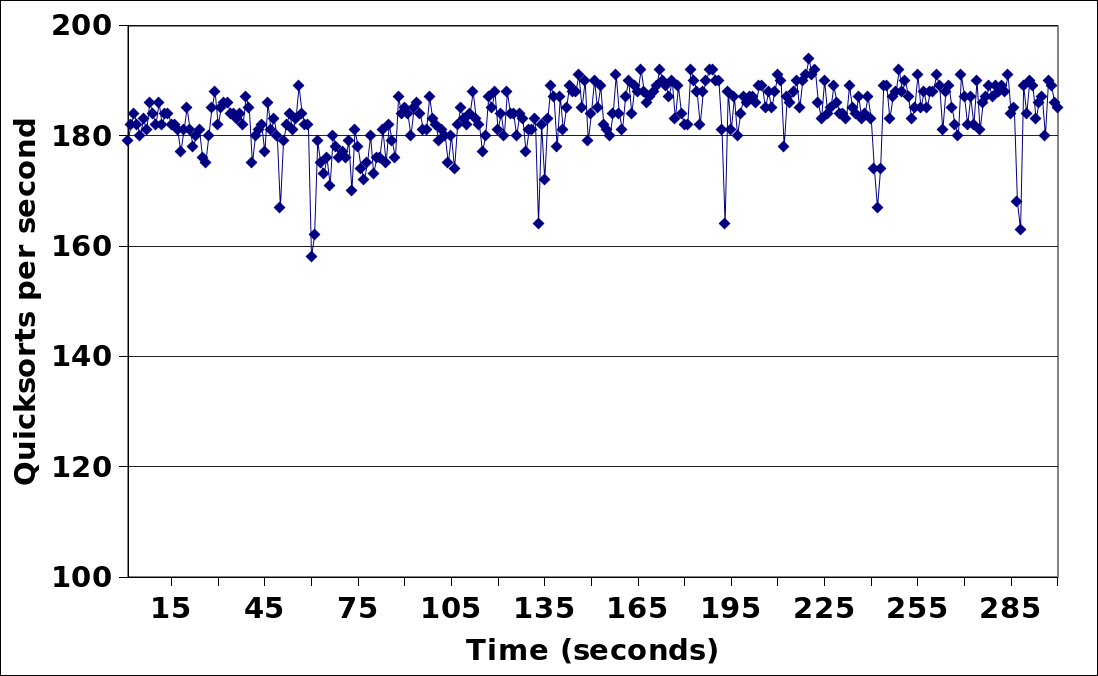
\includegraphics[width=0.5\textwidth]{figures/intrahost-nested-paravirt-quicksort-1GB.png}
%  \caption{Performance of quicksort during migration of a nested guest in para-virtualization %setting}
%  \label{quicksort-performance-1GB-nested-vfio-vhost.png}
%  %\includegraphics[width=15cm,height=6cm,keepaspectratio]{architecture__1_.jpg}
%\end{figure}

%\begin{figure}[t!]
%  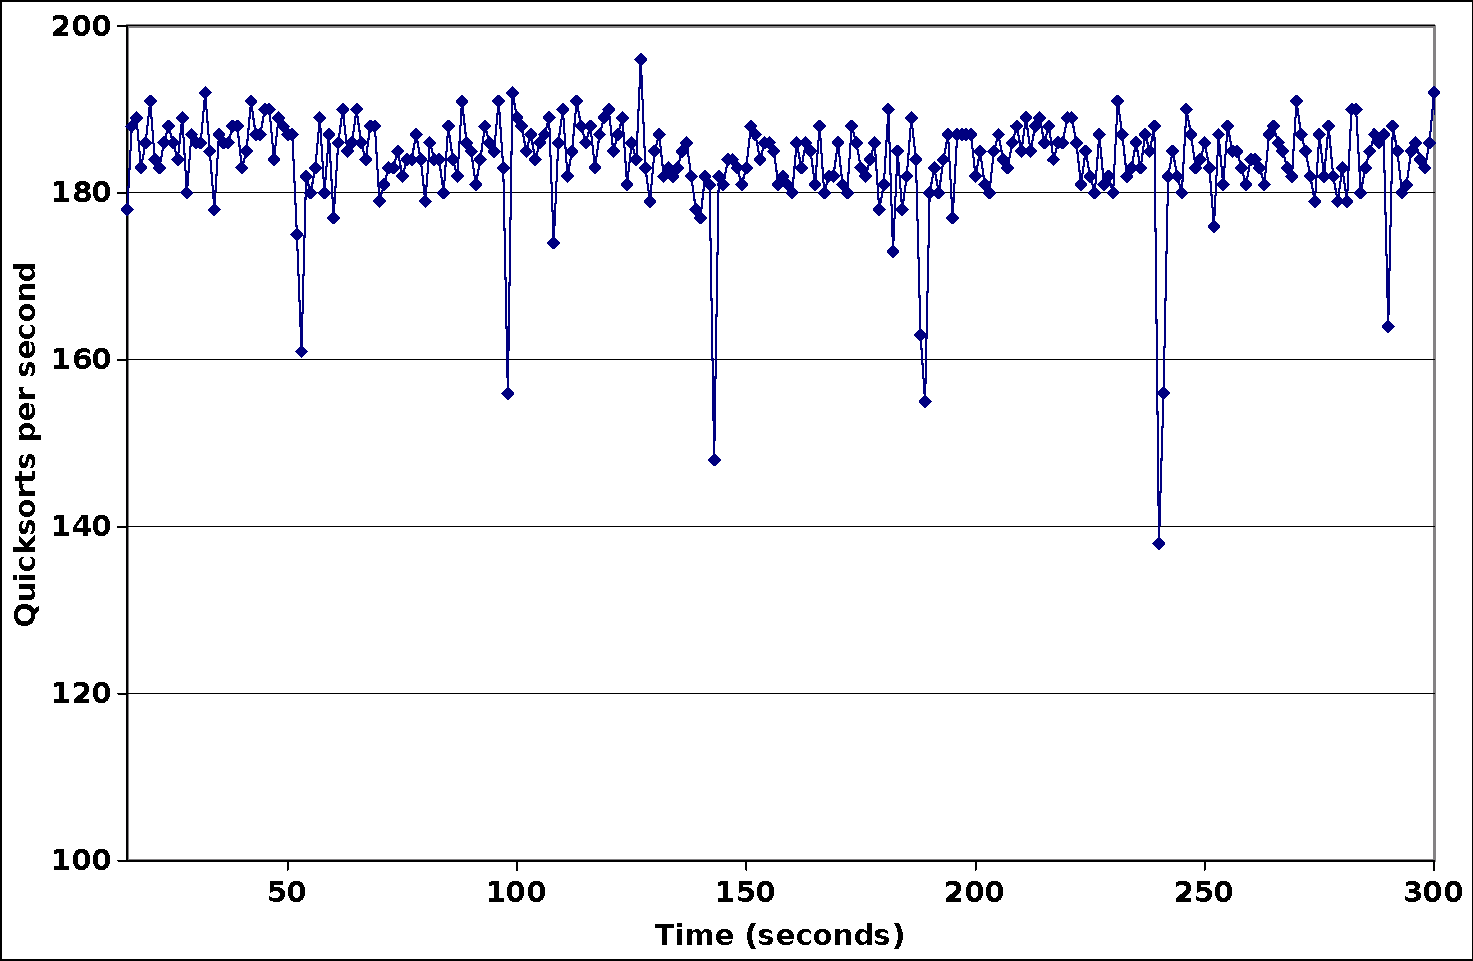
\includegraphics[width=0.5\textwidth]{figures/disable-rate-limit-pre-copy-qsortps-2G.pdf}
%  \caption{Optimized pre-copy live migration: Performance of quicksort during migration of a nested guest}
%  \label{quicksort-performance-1GB-nested-vhost-vhost2.png}
%\end{figure}

%\begin{figure}[t!]
%  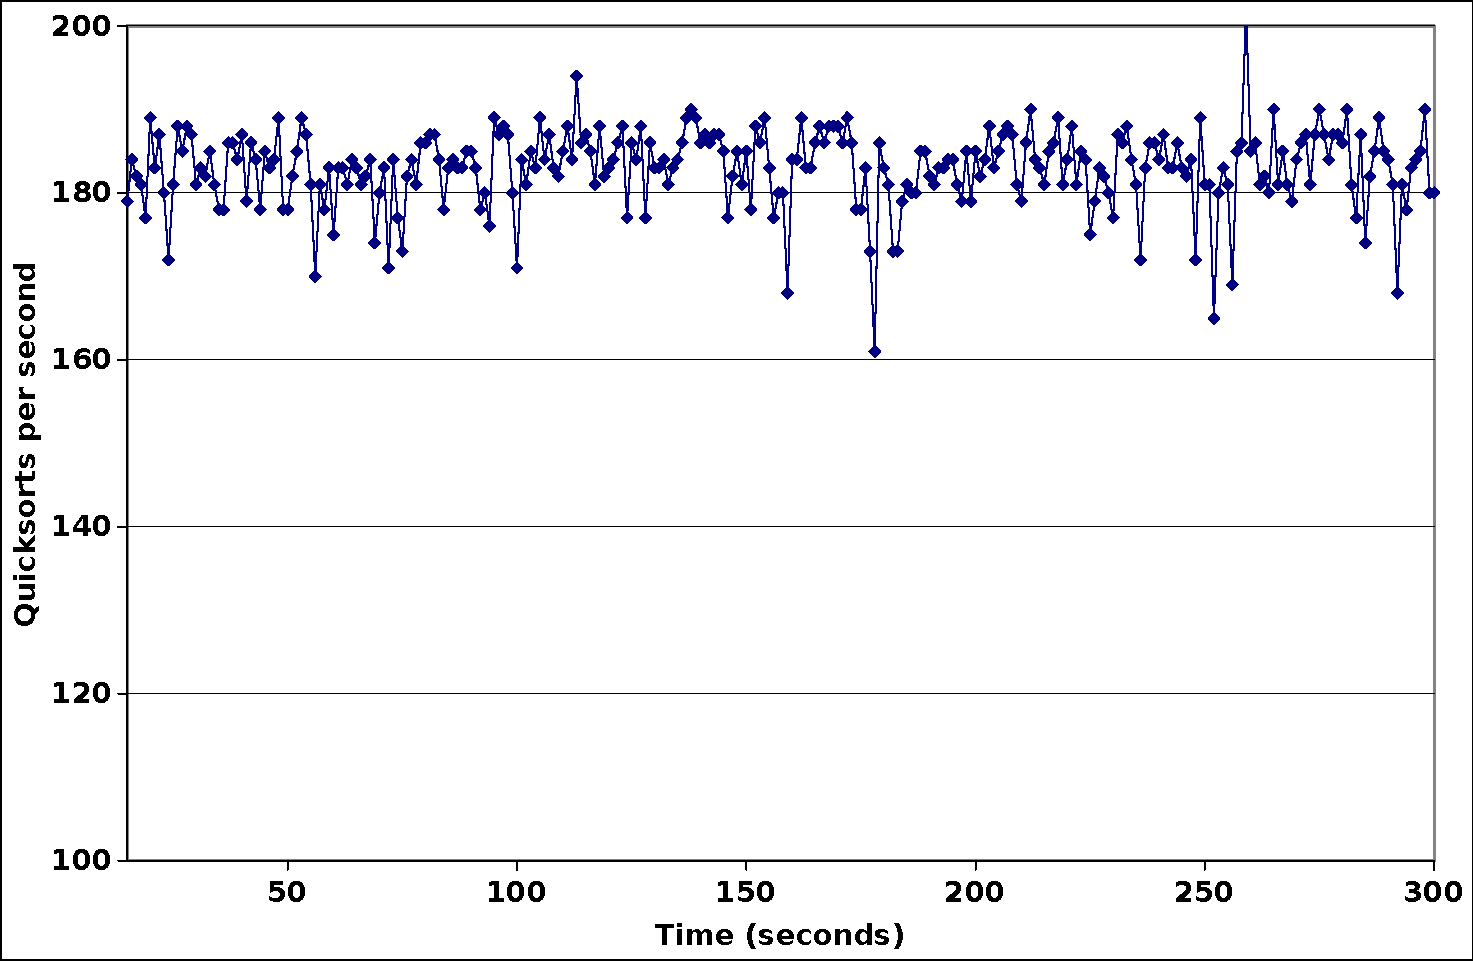
\includegraphics[width=0.5\textwidth]{figures/hyperfresh_qsortps_2G.pdf}
%  \caption{Hyperfresh: Performance of quicksort during migration of a nested guest}
%  \label{quicksort-performance-1GB-nested-vhost-vhost1.png}
%\end{figure}

%Busy guest	Number of Vms variation			
%Guest Memory (GB)			1	    2	    3	    4
%Inter-host					743.6	864.2	940.4	1279.8
%Intrahost non-nested		399.6	449.4	637		906.2
%Intrahost nested (pv-pv)	942.4	1285.8	1419.8	1711.8
%Intrahost nested (pv-pt)	967.4	1182.4	1461.4	1745.8
%Hyperfresh					10		11.6	12		11.4

%\begin{figure}[t!]
%  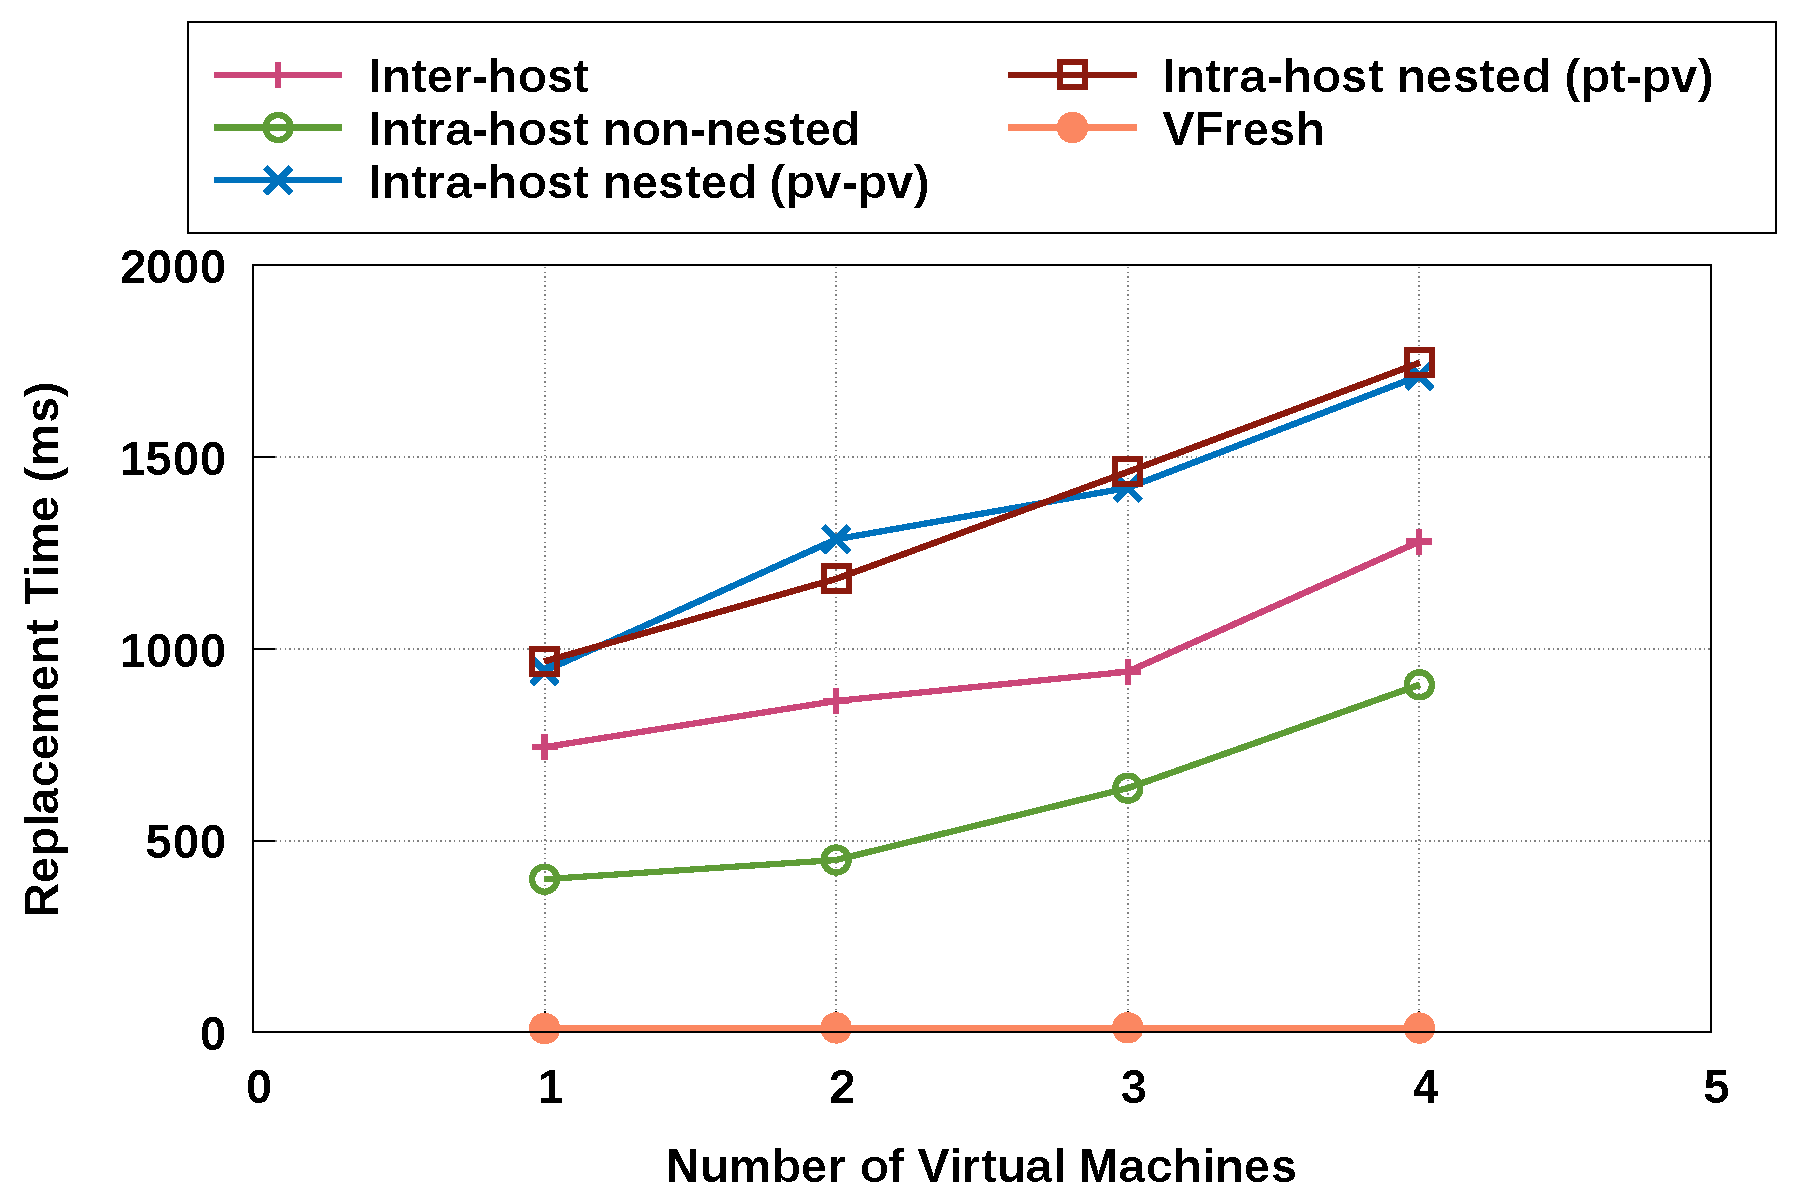
\includegraphics[width=0.45\textwidth]{figures/multivm_busy_guest_migration_vFresh.pdf}
%  \caption{Comparison of hypervisor replacement time for mutiple VMs running write-intensive workloads with \arch and different setups.}
%  \label{fig:multiVfreshBusy}
%\end{figure}

\begin{table}
\small
\begin{tabular}{|p{1.75cm}|p{1.85cm}|p{1.85cm}|p{1.5cm}|} \hline
 & Hyperplexor & Hypervisor & Guest \\ \hline
Host & 8GB, \linebreak 2CPUs & - & - \\ \hline
Non-Nested & 16GB, \linebreak 8CPUs & - & 8GB, \linebreak 2VCPUs \\ \hline
Nested & 32GB,  \linebreak 10CPUs & 16GB, \linebreak 8VCPUs & 8GB, \linebreak 2VCPUs \\ \hline
\arch & 32GB,  \linebreak 10CPUs & 16GB, \linebreak 8VCPUs & 8GB, \linebreak 2VCPUs \\ \hline
\end{tabular}
\raggedright The VM is configured with 4 VCPUs for iperf experiments. The host is also configured with 4 CPUs when iperf is run in host.
\vspace{6pt}
\caption{Experiment setup to measure the performance of Quicksort, Kernbench and iperf benchmarks in the guest.}
\label{tbl:configPerf}
\end{table}

\begin{figure*}
	\centering
    \subfloat[iperf]{
		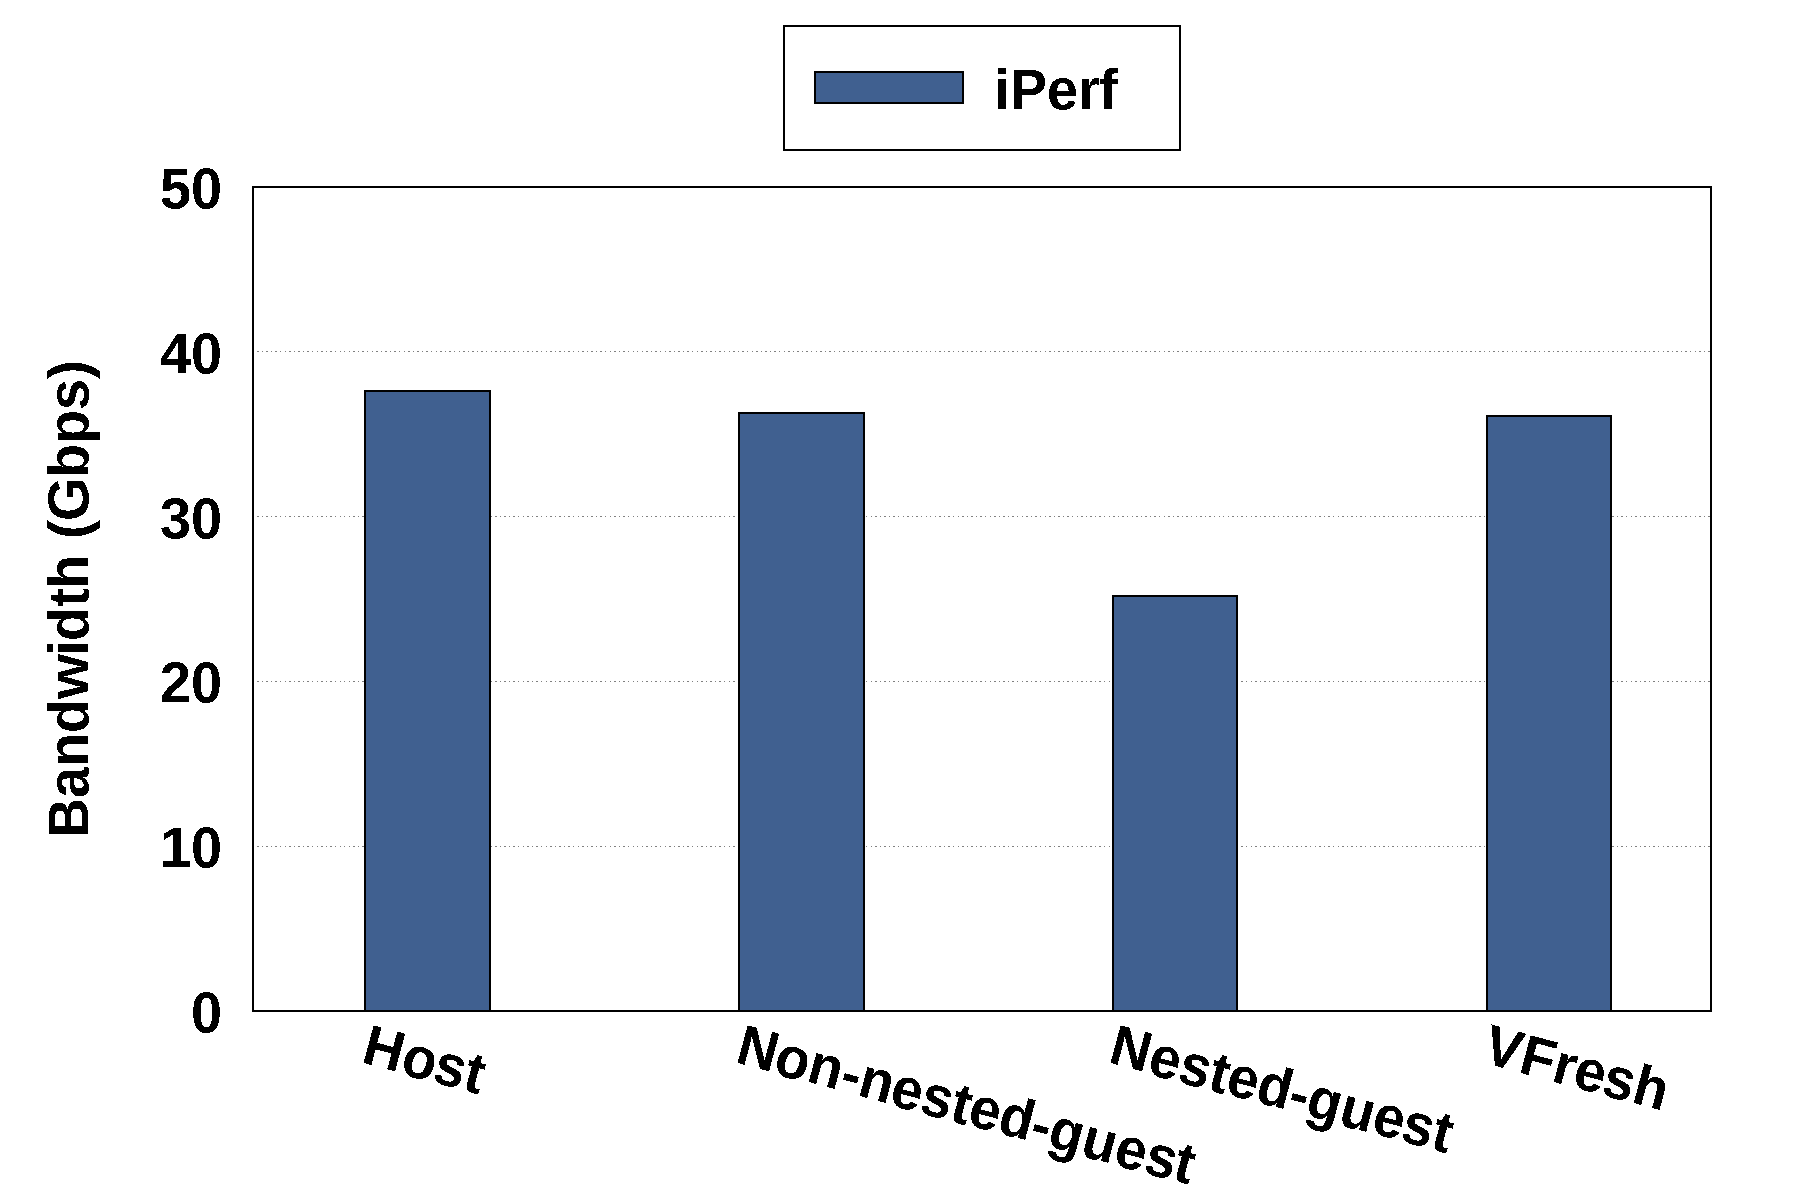
\includegraphics[width=.30\textwidth]{figures/iperf_vFresh.pdf}}
		\hspace{0.1in}
    \subfloat[Kernbench]{
		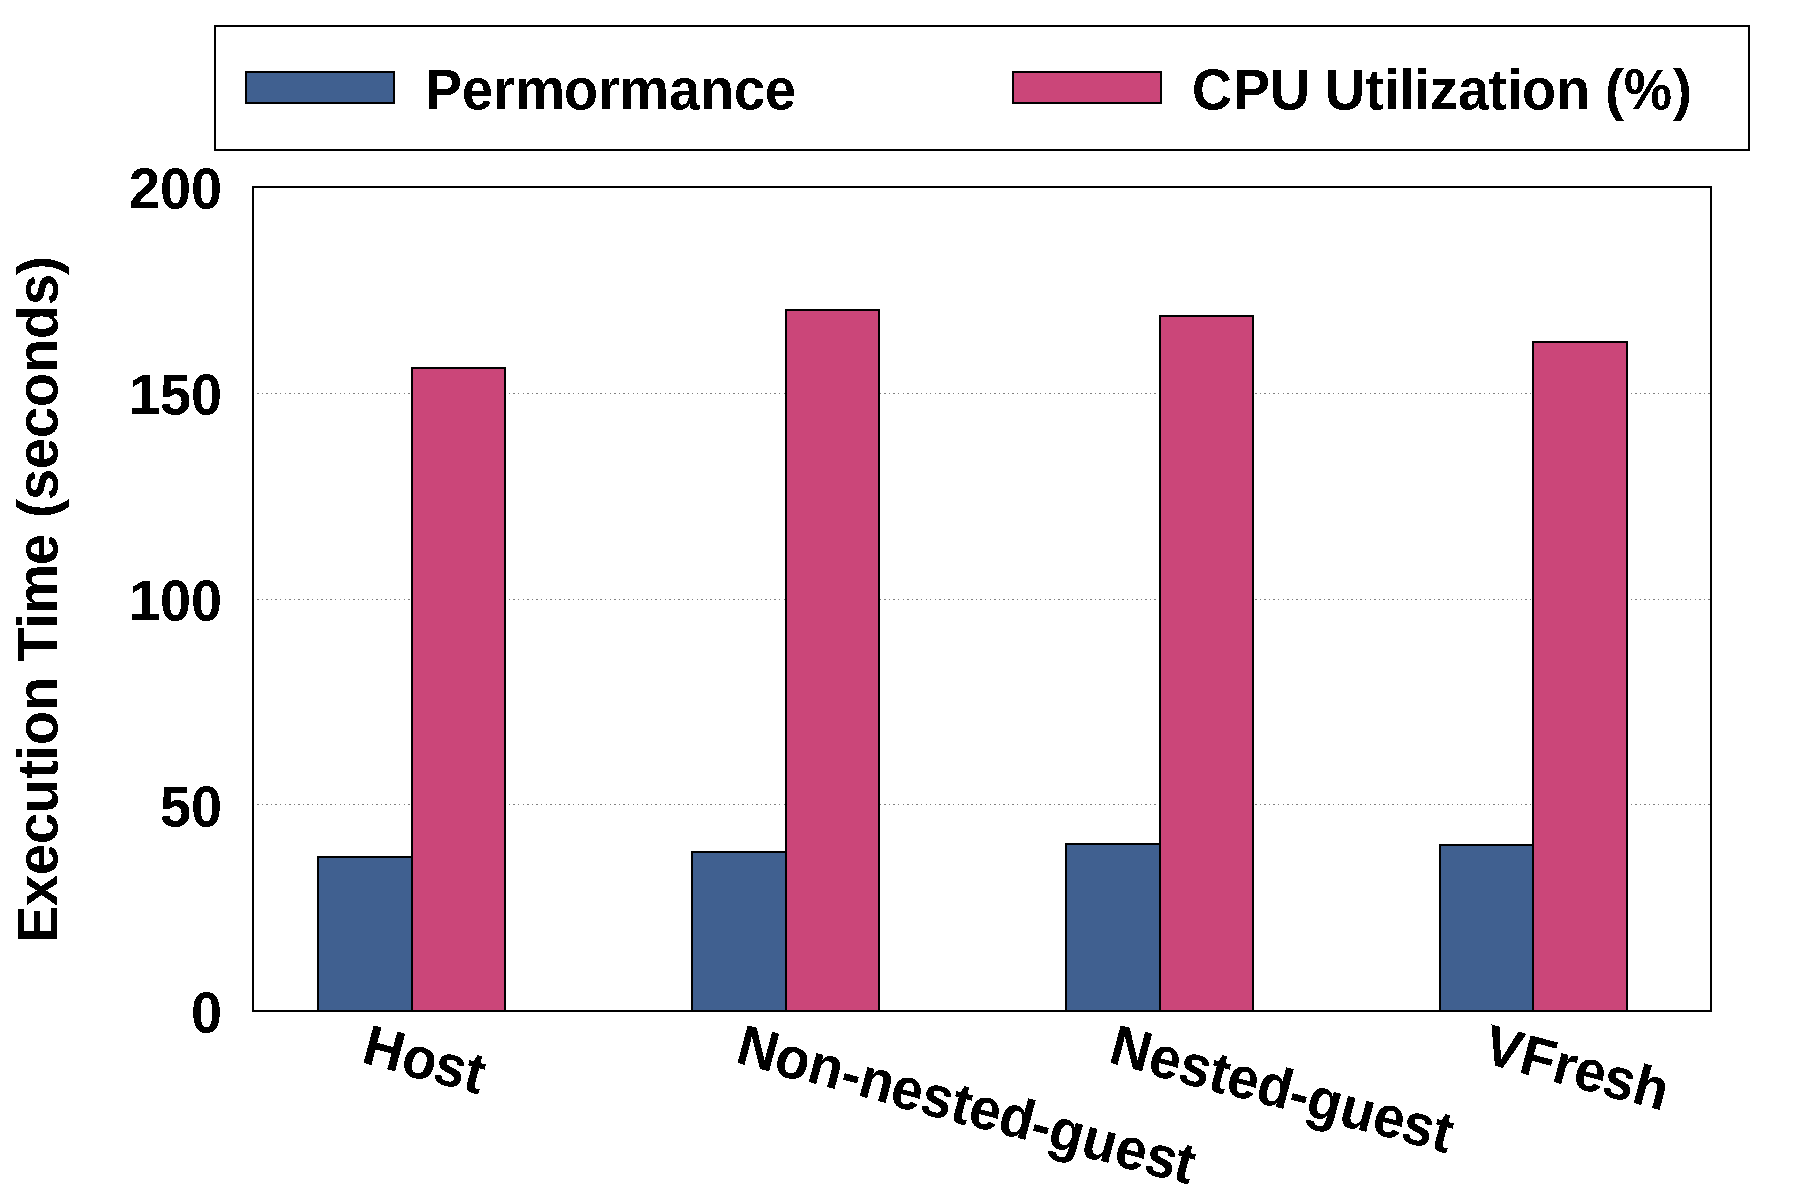
\includegraphics[width=.30\textwidth]{figures/kernbench_vFresh.pdf}}
		\hspace{0.1in}
	\subfloat[Quicksort]{
		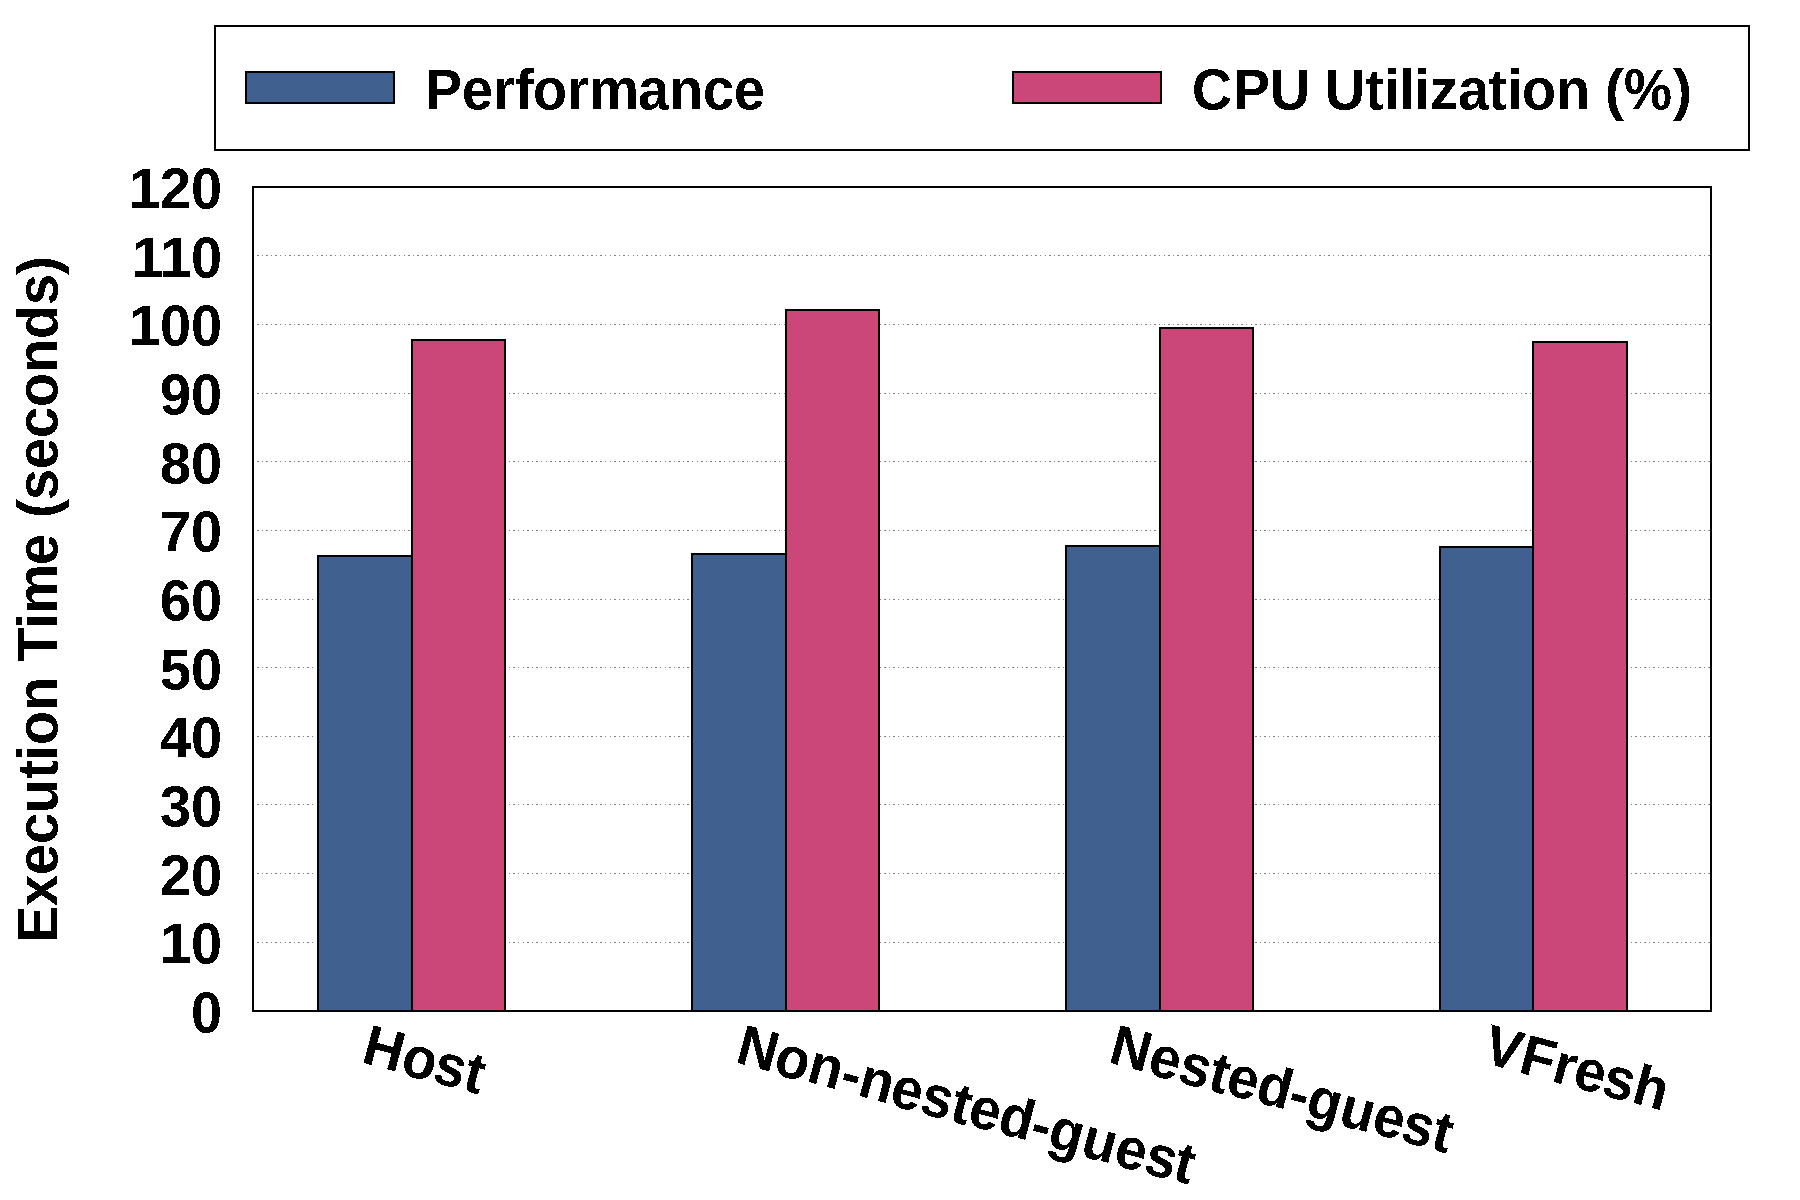
\includegraphics[width=.30\textwidth]{figures/quicksort_vFresh.pdf}}
		%\hspace{0.1in}
    %\subfloat[Breakdown of CPU utilization in system, user modes and guest for iperf benchmark.]{
	%	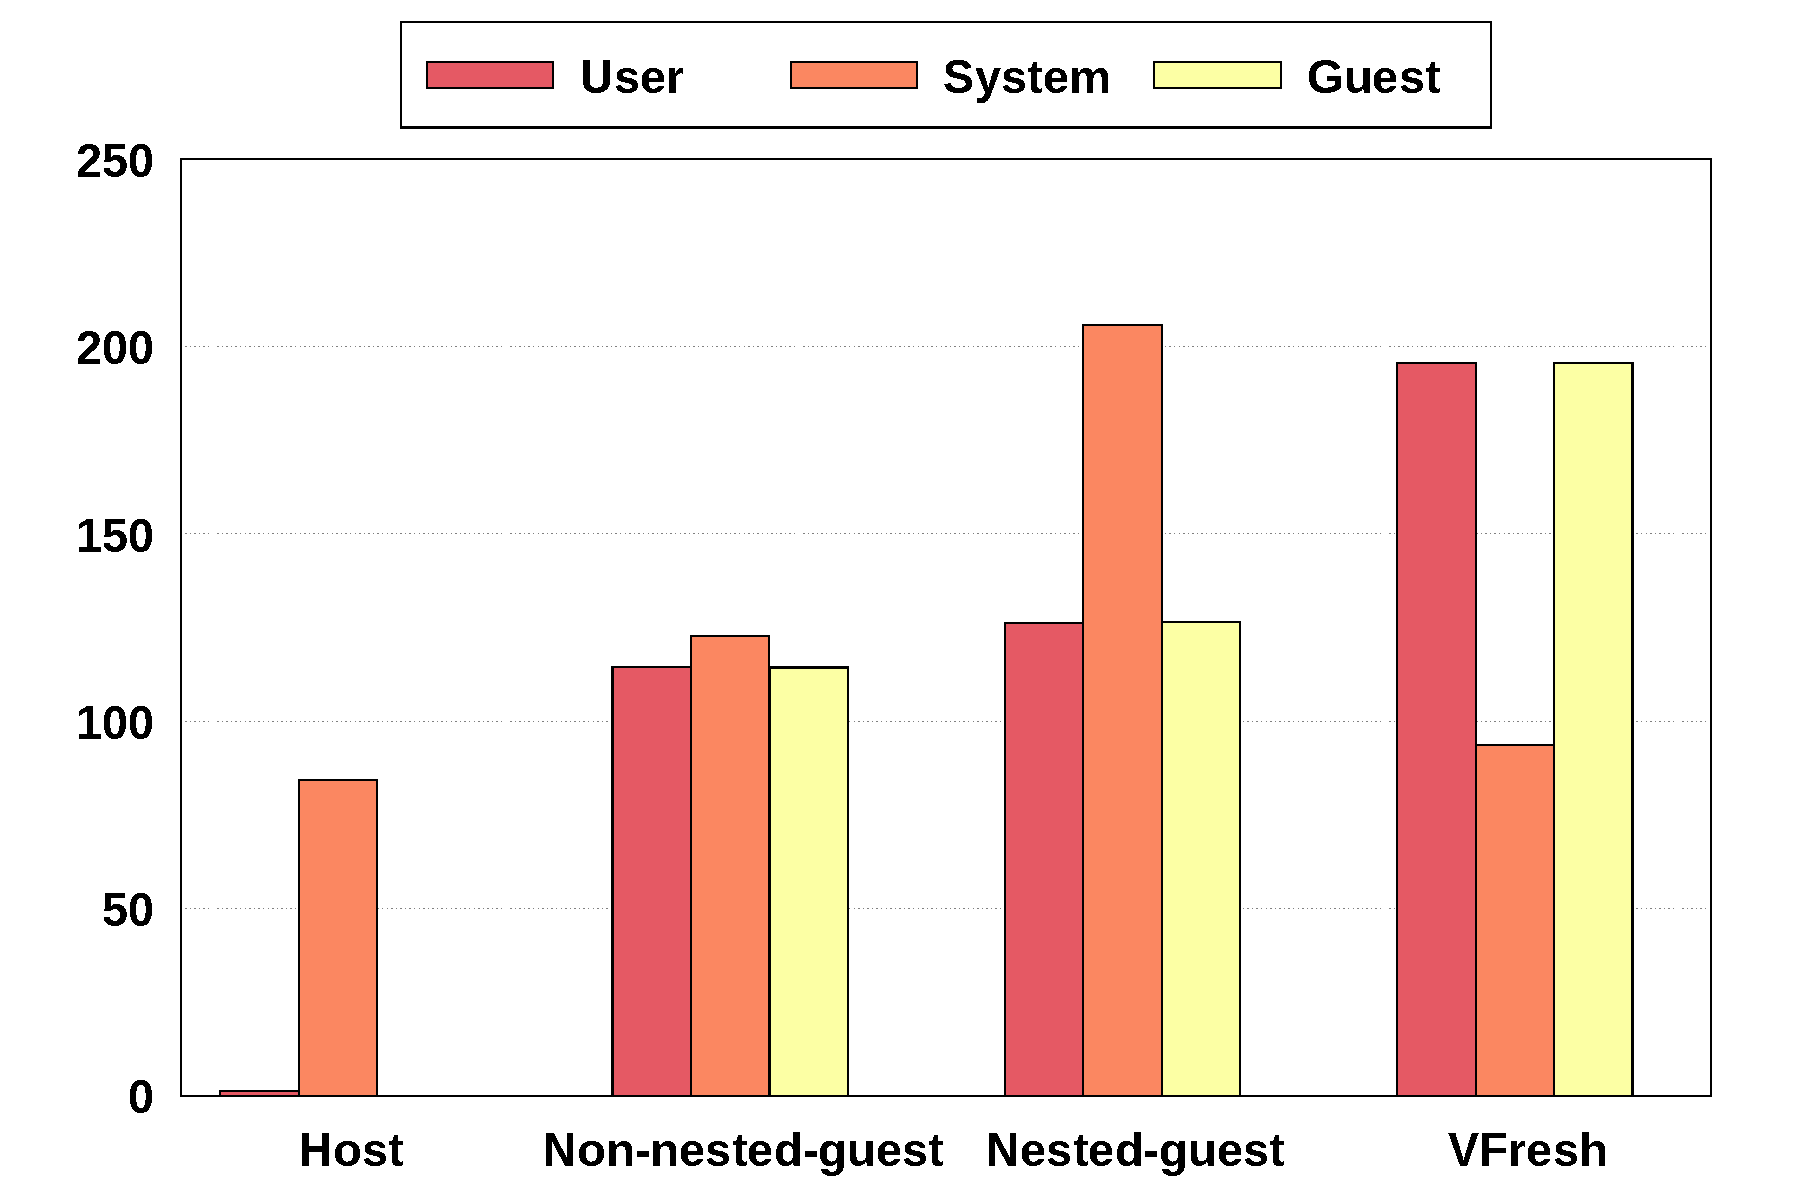
\includegraphics[width=.22\textwidth]{figures/cpu_util_iperf.pdf}}
		%\hspace{0.1in}
		\vspace{-0.1in}
	\caption{Comparison of bandwidth, execution time and CPU utilization on hyperplexor with VFresh and different setups.}
	\vspace{-0.05in}
	\label{fig:impl}
\end{figure*}

\begin{figure}[t!]
  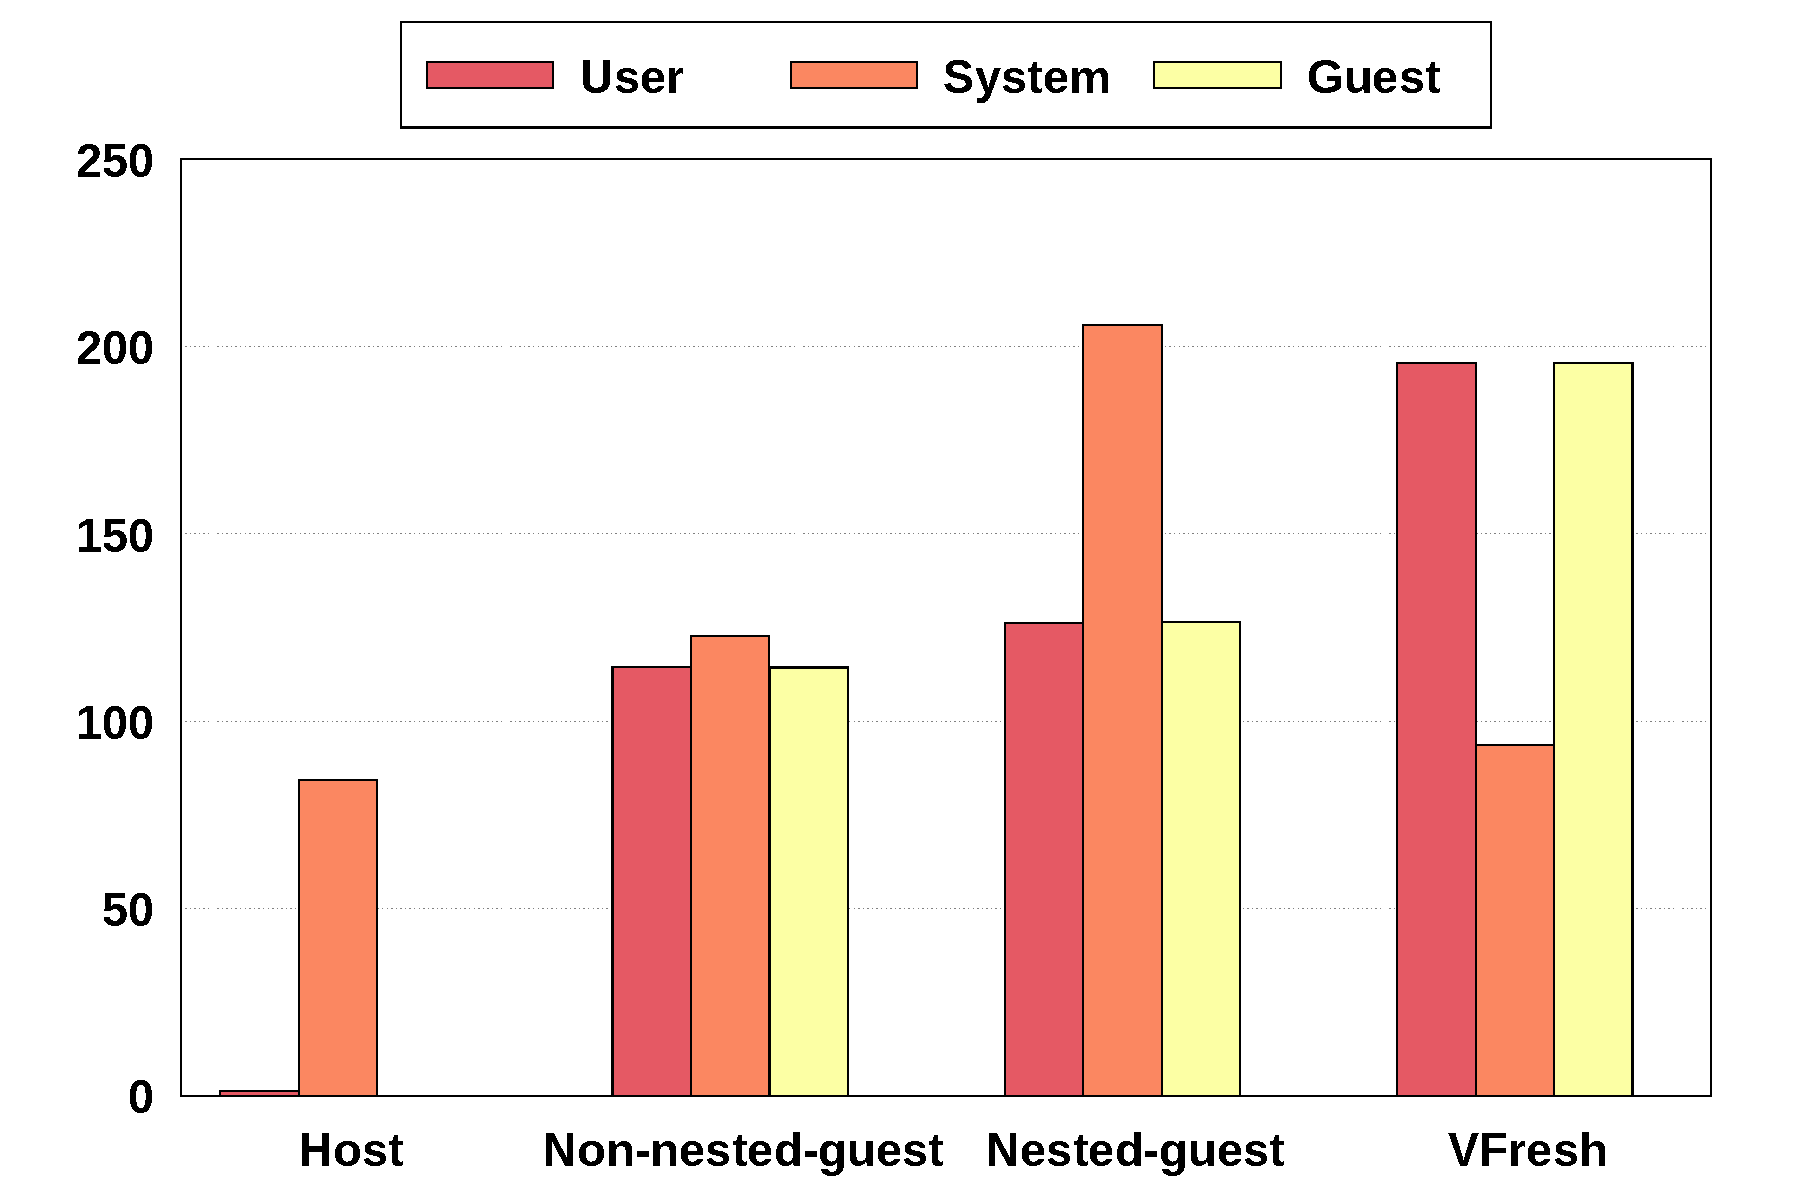
\includegraphics[width=0.33\textwidth]{figures/cpu_util_iperf.pdf}
  \caption{Breakdown of CPU utilization in system, user and guest modes for iperf benchmark.}
  \label{fig:cpuut}
\end{figure}

\subsubsection{Nesting Overhead Mitigation}
To demonstrate the benefits brought by \arch's optimizations to mitigate nesting overhead, we measure the performance of various applications running on (a) the native host (i.e., without virtualization), (b) a VM under non-nested virtualization (with the para-virtualized driver); (c) an L2 VM under nested virtualization (with the pt-pv configuration), and (d) an L2 VM under \arch with optimizations. The configurations for the experiments are listed in Table \ref{tbl:configPerf}. Particularly, to conduct fair comparisons among the above four cases, we ensure that the host or VMs running applications are configured with the same amount of resources --- 2 VCPUs and 8 GB memory. 
%The  performance is measured by running one of the following benchmarks. 
%\begin{itemize}

%\item \textbf{\textit{iPerf}} \cite{iperf} 
\para{Iperf} \cite{iperf} is used to measure network performance. We run the iperf client on the native host or VM under test, and the iperf server on a separate host (with sufficient resources). The iperf client and server are connected via a 40Gbps network. We measure the averaged TCP throughput over 100 seconds. 
%The CPU utilization is further broken down into the user mode, system mode
%due to the network workload in guest.

In \fref{fig:impl}a, we observe that under \arch (with optimizations) the performance of iperf is higher than the default nested case without optimizations, and very close to the non-nested case (under single-level virtualization). 

We also measure the CPU utilization in the hyperplexor, hypervisor and VM, respectively. \fref{fig:cpuut} shows the CPU utilization breakdown in the user mode, system mode the guest (VM) mode. Notice that, the CPU utilization in the user mode also includes the CPU consumed by the VM, while the CPU utilization in the system mode includes the CPU consumed by the hyperplexor (or the native host).

In the default nested case, when the NIC card is assigned to the hypervisor directly (i.e., pass-through), the CPU utilization of the hyperplexor is expected to be small, as the network packets are directly delivered to the L1 hypervisor. However, \fref{fig:cpuut} shows that the CPU utilization of the hyperplexor (i.e., the system mode) in the default nested case is very high. It is because, the hyperplexor burns CPU cycles when it executes HLT instruction as stated in Section \ref{sec:overhead}. In contrast, \arch reduces the CPU utilization of the hyperplexor by disabling \texttt{halt\_poll\_ns}. In consequence, the L1 hypervisor utilizes the CPU more in the VM mode, leading to higher iperf performance than the default nested case. 

%compared to the system mode in hyperplexor.   

%we measure the CPU utilization in hyperplexor while running iperf benchmark in guest. We measure the CPU consumed in user mode, system mode and by the guest separately. 
%The CPU utilization in user mode also includes the CPU consumed by the guest. 
%For a non-nested guest using para-virtual driver, more time is spent in the system to handle the network packets. As a result, the CPU utilization in system mode is high compared to user mode. 
%The CPU utilization of guest is almost equal to the user CPU utilization indicating that the guest is utilizing the CPU for the rest of the time. 
%When NIC card is assigned to the hypervisor, the CPU utilization in the hyperplexor is expected to be less as the network packets are directly delivered to the hypervisor. But the CPU utilization in hyperplexor is high as the hypervisor VCPUs burn CPU cycles when they execute HLT instruction. The nested guest uses para-virtual driver to handle the network traffic. The CPU utilization in the system mode in the hypervisor is higher than the CPU utilization in guest or user mode. In VFresh, we reduce the CPU utilization in system mode in hyperplexor by disabling halt\_poll\_ns. As seen from the results, the hypervisor now utilizes the CPU more in guest mode compared to the system mode in hyperplexor.   


%\item \textbf{\textit{Kernbench}} 
\para{Kernbench} \cite{kernbench} is a CPU and I/O intensive benchmark, which uses multiple threads to compile the kernel source code. More specifically, the benchmark fetches kernel source code files from disk for compilation and writes the binary files back after compilation. For our experiments, the kernel is compiled for five iterations and the number of threads used to perform kernel compilation is set to 2, equal to the number of VM VCPUs. 

In \fref{fig:impl}b, the non-nested VM brings 2.8\% performance overhead in comparison with the native case due to the single-level virtualization overhead; the default nested VM introduces 8.1\% overhead in comparison with the native case due to the additional layer in nested virtualization. %why 
\arch slightly reduces the overhead by 6\% and consumes less CPU in comparison with the default nested case.

\para{Quicksort} is a memory and CPU-intensive benchmark, as stated above. In \fref{fig:impl}c, the non-nested VM introduces only 0.3\% performance overhead in comparison with the native case; the default nested VM introduces 2.23\% overhead in comparison with the native case. %why 
Again, \arch slightly reduces the overhead by 15\% and consumes less CPU utilization in comparison with the default nested case.

%quicksort benchmarks causes overhead of 7.6\% and 1.9\% for kernbench and quicksort respectively, which do not show significant improvement. However, the performance does not degrade due to the optimizations applied. 

%\item \textbf{\textit{Quicksort}} 
%\para{Quicksort} \cite{williams2016enabling} is a memory and CPU-intensive benchmark. In the first stage, Quicksort allocates 1GB memory using malloc() system call. In the second stage, it writes random integers in the allocated memory and performs sorting operations using quicksort algorithm. In our experiments we measure the total number of sorting operations per second.


%\begin{table*}\centering
%\begin{tabular}{|p{4.5cm}|p{0.8cm}|p{0.8cm}|p{0.8cm}|p{0.8cm}|p{0.8cm}|p{0.8cm}|p{0.8cm}|p{0.8cm}|p{0.8cm}|p{0.8cm}|} \hline
%    \multirow{1}{*}{} & &
%      \multicolumn{9}{c|}{CPU Utilization} \\ \cline{3-11}
%    \multirow{1}{*}{} & Guest &
%      \multicolumn{3}{c|}{Hyperplexor} & 
%      \multicolumn{3}{c|}{Hypervisor} & 
%      \multicolumn{3}{c|}{Guest} \\ \cline{3-11}
 %& \multicolumn{9}{|c|}{\textbf{CPU Utilization (\%)}} \\ \cline{2-10}
 %& \multicolumn{3}{|c|}{\textbf{Host (\%)}} \\ \cline{2-4} 
% \multicolumn{3}{|c|}{\textbf{L1 (\%)}} \\ \cline{5-7}
% \multicolumn{3}{|c|}{\textbf{Guest (\%)}} \\ \cline{8-10}
% & \textbf{CPU Utilization on Host (\%)} \\ \hline
%\textbf{} & & User & System & Guest & User & System & Guest & User & System & Guest \\ \hline
%\multirow{ 2}{5cm}{Non-nested guest (pv)} & Server & 114.63 & 247.09 & 114.63 & - & - & - & 1.8 & 91.7 & 0 \\ 
%& Client & 114.4 & 122.7 & 114.3 & - & - & - & 1.18 & 84.64 & 0 \\ \hline

%\multirow{ 2}{5cm}{Nested Guest (pt-pv)} & Server & 253.1 & 308.3 & 252.9 & 91.18 & 150.72 & 90.9 & 1.9 & 107.18 & 0\\ 
%& Client & 126.3 & 205.7 & 126.5 & 82.72 & 107.54 & 82.63 & 0.63 & 121.17 & 0 \\ \hline

%\multirow{ 2}{5cm}{\arch} & Server & 265.7 & 85.5 & 265.7 & 116.2 & 143.1 & 116.45 & 2.45 & 118.44 & 0 \\ 
%& Client & 195.6 & 93.5 & 195.6 & 95.54 & 93.18 & 95.27 & 1.17 & 135.8 & 0 \\ \hline

%\end{tabular}
%\vspace{6pt}
%\caption{CPU Utilization: }
%\label{tab:cpuut}
%\end{table*}


%Fig.11 c explanation
%In our experiments, we disable the halt_poll_ns parameter.  In nested virtualization experiments, mainly network experiments (iperf), we assign 8 vCPUs to L1 hypervisor and 4 vCPUs to L2 guest and the host has 10CPUs. As we isolate and pin L1 vCPUs to pCPUs, 8 pCPUs are occupied and other 2 pCPUs are dedicated for QEMU and other I/O threads associated with QEMU. When the interrupt has to be delivered to L2 guest vCPUs, L2 has to be scheduled on pCPUs first, by pre-empting L1 vCPU on which it was running. If halt_poll_ns is 0, L1 vCPU will execute HLT instruction faster and the L0 scheduler schedules L2 vCPU and interrupt gets delivered faster. 
%That way, the network performance becomes better in our solution using nested virtualization.

%KERNBENCH
%host - 2 CPUs, 8G
%37.47
%single-level, vhost-net , 8 CPUs, 2 vCPUs, 16G, 8G
%38.51
%nested, passthrough-vhost, 10CPUs, 8vCPUs, 2 vCPUs
%40.524
%VFresh
%40.324

%CPU Utilization
%host - 155.95
%single-level - 170.12
%nested, passthrough-vhost - 168.7
%VFresh - 168.5

%QUICKSORT
%host - 2 CPUs, 8G
%66.29
%single-level, vhost-net , 8 CPUs, 2 vCPUs, 16G, 8G
%66.51
%nested, passthrough-vhost, 10CPUs, 8vCPUs, 2 vCPUs
%67.77
%VFresh
%67.57

%CPU Utilization
%host - 97.71
%single-level - 102.1
%nested, passthrough-vhost - 99.4
%VFresh - 97.5

%IPERF
%host - 2 CPUs, 8G
%SENDER: 37.6 Gbps RECEIVER: 37.6 Gbps
%single-level, vhost-net , 8 CPUs, 2 vCPUs, 16G, 8G
%SENDER: 36.3 Gbps RECEIVER: 29.9 Gbps
%nested, passthrough-vhost, 10CPUs, 8vCPUs, 2 vCPUs
%SENDER: 25.2 Gbps RECEIVER: 26.6 Gbps
%nested, passthrough-vhost, 10CPUs, 8vCPUs, 2 vCPUs + optimizations

%\end{itemize}

%In Table 1 we measure the performance overhead caused due to virtualization. We compare the overhead caused due to nested virtualization with non-nested virtualization. In our proposed solution we measure the performance by applying the following optimizations for nested case. The 8 VCPUs of hypervisor are pinned to 8 CPUs, CPUs are isolated so that any other process other than VCPU does not get scheduled on CPU. 1 CPU is dedicated to schedule hypervisor and QEMU threads.The NIC card is directly assigned to hypervisor and halt\_poll\_ns is set to zero in hyperplexor. For nested case, we passthrough the NIC card to hypervisor and the guest uses para-virtualized driver.

%In \fref{fig:impl} (b), for non-nested guest, to measure the iperf performance the guest is configured with para-virtualized driver. 
%The performance of iperf is 36.3 Gbps for a 40 Gbps NIC card when iperf client is run in guest. However, the performance reduces to 29.9 Gbps when iperf server is run in the guest. The loss in performance is due to the processing of huge number of incoming packets. When iperf is run in nested guest the performance reduces to 25.2 Gbps. %why
%In our solution, as the halt\_poll\_ns is disabled in the hyperplexor, the CPU scheduler gets invoked and schedules the nested guest VCPUs sooner to handle the interrupts. As a result the performance of iperf is now comparable with the performance in the single-level guest.

%\begin{figure}[t!]
%  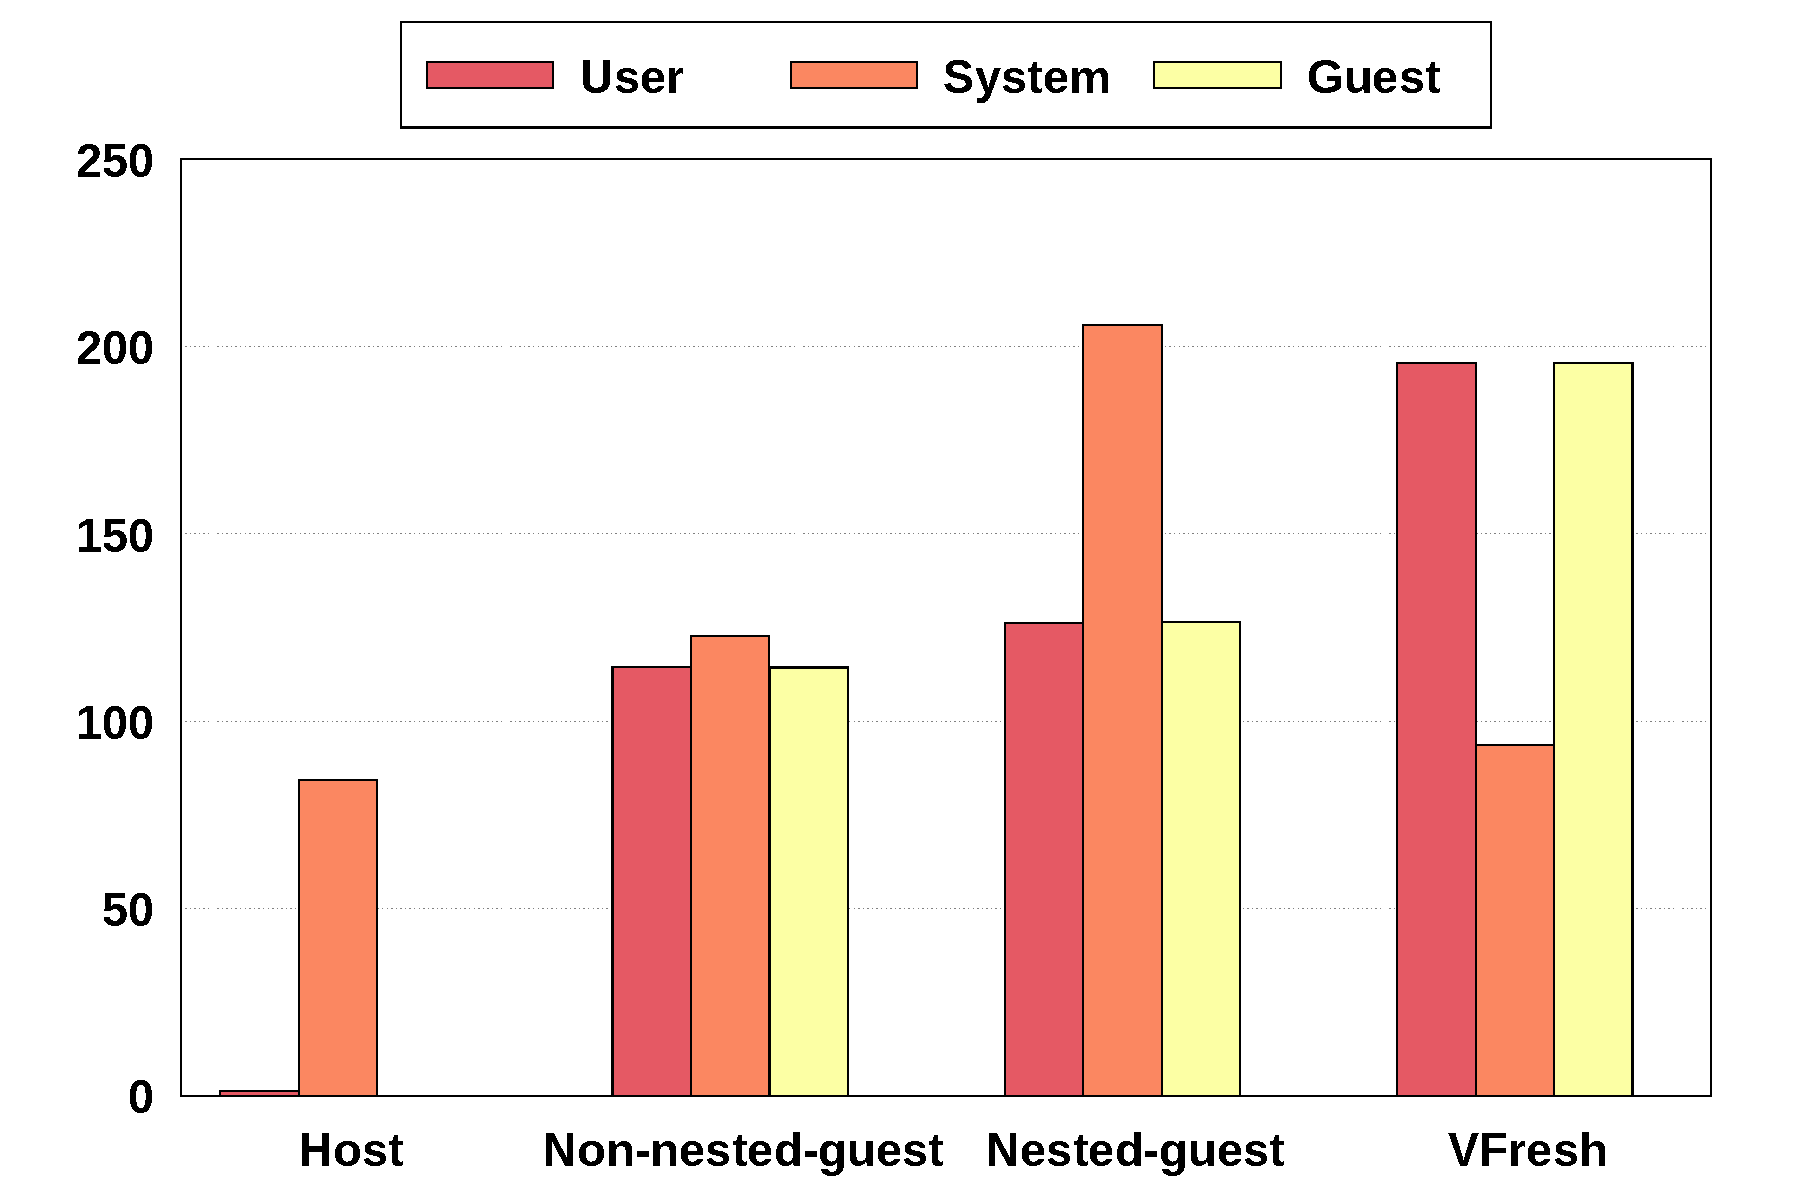
\includegraphics[width=0.45\textwidth]{figures/cpu_util_iperf.pdf}
%  \caption{Breakdown of CPU utilization in system, user modes and guest for iperf benchmark.}
%  \label{fig:cpuut}
%\end{figure}


%The performance of kernbench and quicksort introduces 2.8\% and 0.3\% overhead respectively in non-nested guest compared to host, whereas the nested guest introduces 8.1\% and 2.23\% overhead due to the additional layer of virtualization. %why 
%With our proposed solution the performance of kernbench and quicksort benchmarks causes overhead of 7.6\% and 1.9\% for kernbench and quicksort respectively, which do not show significant improvement. However, the performance does not degrade due to the optimizations applied. 


%\begin{figure} 
%	\centering
%	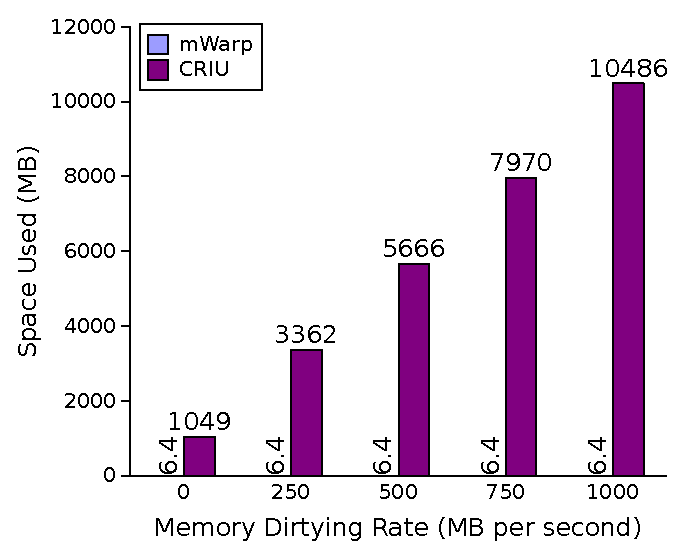
\includegraphics[width=0.5\textwidth]{figures/space_used.eps}
%	\caption{Space Used For Migration}
%	\label{fig: spaceused}
%\end{figure}
